\def\year{2017}\relax
%File: formatting-instruction.tex
\documentclass[letterpaper]{article}
\usepackage{aaai17}
\usepackage{amsmath}
\usepackage{amsthm}
\usepackage{times}
\usepackage{helvet}
\usepackage{courier}
\usepackage{graphicx}
\usepackage{subfigure}
\usepackage{mdwmath}
\usepackage{mdwtab}
\usepackage{amssymb}
\usepackage{booktabs}
\usepackage{algorithm}
\usepackage{pifont}
\usepackage[noend]{algpseudocode}
\usepackage{balance}
\usepackage{bm}
\usepackage{ulem}
\usepackage{array}
\usepackage{balance}
\usepackage{multirow}
\usepackage{multicol}
\frenchspacing
\setlength{\pdfpagewidth}{8.5in}
\setlength{\pdfpageheight}{11in}
\usepackage[marginal]{footmisc}
\pdfinfo{
/Title (EUI: A General Framework of the Reduced Variance Stochastic Gradient Descent and the Accelerated Implementation )
/Author (Yawei Zhao)}
\setcounter{secnumdepth}{0}  
 \begin{document}
% The file aaai.sty is the style file for AAAI Press 
% proceedings, working notes, and technical reports.
%
\title{EUI: A General Framework of the Reduced Variance Stochastic Gradient Descent and the Accelerated Implementation}
%\author{
%}
\maketitle
\begin{abstract}
Stochastic gradient descent (SGD) with the variance reduction  technique is efficient to train parameters of many machine learning algorithms. Although many variants of SGD with the variance reduction technique have been proposed,  the analysis of variance does not gain enough discussion, and thus the power of the variance reduction technique is not exploited. In this paper, we propose a general framework denoted by \emph{EUI}  to unify the existing versions of SGD with the variance reduction technique, and then  provide a fine-grained analysis of the variance from a new prospective. Moreover,  since the variance reduction technique needs a snapshot of the full gradient  for every epoch, which is time-consuming, a new variant of SGD with the variance reduction technique denoted by \emph{EstimateVR} has been proposed. \emph{EstimateVR} uses the estimation of the full gradient instead of computing it, thus accelerating the convergence of the training loss. 
The theoretical analysis shows 

 and gains the linear convergence rate.  Both the theoretical and the empirical studies have verified that EstimateVR outperforms other previous work. 
\end{abstract}

\section{Introduction}
\label{sect_introduction}
Many machine learning problems such as classification and regression  can be  presented like the optimisation problem in Equation \ref{equa_loss_minimization}. $\omega$ is the parameter of a machine learning model. $F(\omega)$ is the loss function which is the sum of the finite functions, i.e. $f_i(\omega)$. $R(\omega)$ is the regulariser  which is used to prevent overfitting.    

\begin{equation}
\label{equa_loss_minimization}
\min F(\omega),~~~~~F(\omega)=\frac{1}{n}\sum\limits_{i=1}^n f_i(\omega)+R(\omega)\\
\end{equation}. 

Gradient descent (GD) is often used to train the parameters in such underlying machine learning problems. Since GD computes the full gradient  in each iteration, it leads to extremely large amount of derivative calculations unavoidably. With the proliferation of training data, GD is not efficient to train parameters for a large scale machine learning task. The stochastic gradient descent (SGD) overcomes the disadvantage of GD by using a stochastic gradient instead of the full gradient to train parameters. However, the variance of the optimisation objective due to the stochastic gradient usually impairs the convergence of parameters during the training process. Specifically, when the parameter is close to the optimum, it is more and more difficult to made a further progress  due to the variance.

Conventional studies show that a decaying learning rate can be used to decrease the variance. However, the decaying learning rate usually slows the convergence of the loss function, when the learning rate has been decreased to a tiny value. Recently, Johnson et al. improves SGD with the variance reduction technique denoted by \emph{SVRG} which uses a constant learning rate to train the parameter \cite{Johnson:9MAvkbgy}. SVRG is organised by epochs, and each of which consists of a number of iterations.  Based on the variance reduction technique adopted by SVRG, many variants of SVRG such as S2GD \cite{Richtarik:2013te}, mS2GD\cite{Liu:2015bx}, EMGD \cite{Zhang2013Linear}, SVR-GHT \cite{Li:2016vh}, Prox-SVRG \cite{Xiao:2014vw}, SVRG++ \cite{Allen2015Improved}, Katyusha \cite{Allenzhu2016Katyusha} have been proposed. Those achievements use the variance reduction technique, but accelerate SVRG by using a weak assumption, or apply it in different scenarios. However,  the variance and the potential of the variance reduction technique lack of enough discussion. Since the variance reduction technique is designed  to reduce the variance caused by the stochastic gradient, it is meaningful to measure and give the quantitative analysis  of the variance so that the potential of the variance reduction technique can be exploited.  Additionally, the variance reduction technique needs a snapshot of the full gradient at the beginning of an epoch, which consumes much time. If the snapshot of the full gradient can be avoided, those versions of the reduced variance will be accelerated a lot, and achieve a better performance of the convergence.
 
Comparing with SGD and GD, we  understand the reason of the underlying variance reduction technique from a new prospective. The  update gradient by using variance reduction technique can be divided into three ingredients, including the variance source, the variance reducer and the progressive direction. Specifically, the variance reducer is the real reason to reduce the variance. From the analysis of the variance reducer, we find that the source of the variance is introduced from  the distance between the current and  the expected state of the parameter. The analysis is applied to the existing versions of SGD with the variance reduction technique in order to provide an entire understand of these achievements. Moreover, we design a new version SGD with the variance reduction technique, which replaces the snapshot of the full gradient by an unbiased estimate of the  full gradient, and gains the linear convergence. Such the unbiased estimate of the full gradient sharply decreases the time consumption caused by  the full gradient.

To present our analysis about the variance, we first present an unified  framework, i.e. \emph{EUI}  which can express various of the  existing variants. EUI mainly consists of three ingredients which should be considered when  designing a good variant of SGD with the variance reduction technique. After analysing the variance in quantitative,  the guide to design a good version of SGD has been provided. Furthermore, a new version of reduced variance SGD, i.e. EstimateVR has been proposed, and the convergence performance of EstimateVR has been analysed in theroetical. Finally, the extensive empirical studies verify that EstimateVR outperforms than the existing methods. The contributions of the paper are outlined as follows:

\begin{itemize}
\item The variance caused by the stochastic gradient in the underlying framework is analysed in quantitative. A lower bound of the variance is presented.
\item A general framework, i.e. EUI is proposed to unify the existing variants of reduced variance SGD. The variance of the previous work has been analysed by using this framework.
\item A new version of SGD with the variance reduction technique, i.e. EstimateVR is been proposed, which replaces the snapshot of the full gradient by using an estimate via a sampling strategy.
\item The theoretical and extensive numerical evaluations verify that EstimateVR outperforms than other previous work significantly. 
\end{itemize}
 
The paper is organised as follows. Section \ref{ sect_related_work } reviews the recent work about SGD with the variance reduction technique. Section \ref{sect_framework}  presents the general framework, i.e. EUI which unifies almost all the existing variants of SGD with the variance reduction technique. Section \ref{sect_variance_analysis} analyses the variance of the previous work under the framework. Section \ref{sect_EstimateVR} presents a new reduced variance SGD.   Section \ref{sect_performance_evaluation} demonstrates the extensive performance evaluations to verify our theoretical analysis. 
 

\section{Related work}

\label{sect_related_work}

\section{EUI: the general framework of reduced variance SGD}
\label{sect_framework}
\subsection{Framework}
We present a general framework denoted by EUI which contains a loop of the epochs. As illustrated in Algo. \ref{algorithm_EUI}, an epoch consists of a number of iterations. EUI first identifies the sampling strategy by a probability distribution. Generally, the probability distribution is uniform so that the training data will be picked uniformly. The epoch size then is required to be identified, which is represented by the function $\mathcal{E}$. The size of an epoch will be shown to have  a great impact on the variance, but it is non-trivial to identify a good value. Additionally, the function $\mathcal{U}$ stands for the update rule during the train of the parameter. A sequence of the local parameters, i.e.  $\omega_{i_{j}}^t$ with $j\in\{1,2,..., m_s\}$ is obtained by performing the update of the parameter in an epoch. When the inner loop is completed, the global parameter $\omega^s$ will be updated by the sequence of the parameter $\omega_{i_{j}}^t$ with $j\in\{1,2,..., m_s\}$, which is shown by the function $\mathcal{I}$. 

The general framework is powerful so that almost all the existing versions of SGD with the variance reduction technique except for SAG \cite{Schmidt:2013ui} and SAGA \cite{Defazio:2014vu}. SAG and SAGA can be expressed by EUI with a little change. To keep the simplicity, we do not unify them into the framework, but the analysis of the variance in the following part will contain them. The Fig. \ref{figure_EUI_example} illustrates that existing versions of reduced variance SGD can be expressed by EUI by implementing the specific functions. Compared to the basic version, i.e. SVRG, the following algorithms implement those functions by using different strategies in order to improve SVRG. For example, SVRG achieves the linear convergence when the loss function $F(\omega)$ is Lipschitz-continuous, and the functions $f_i(\omega)$ with $i\in\{1,2,...,n\}$ are strongly convex. However, these assumptions can be relaxed to solve the non-strongly convex objective by designing different strategies and implement those functions. 

\begin{algorithm}[t]
    \caption{The general framework of variance reduced SGD: EUI}
    \label{algorithm_EUI}
    \begin{algorithmic}[1]
        \Require $\omega^0\in \mathbb{R}^d$. $\forall i\in[n]$, and $[n]$ represents $\{1,2, ..., n\}$.
        \State $P(i_t)\leftarrow \frac{1}{n}$ where $i_t \in \{1,2, ..., n\}$. $t$ is a positive integer;
        \State \textbf{\uline{E}poch:} the sequence of the epoch size $\{m^0, m^1, ..., m^S\}\leftarrow \mathcal{E}([i_t])$;
        \For {$s=0,1,2,...,S$}
            \State $\omega_0^s=\tilde{\omega}^s$;
            \State $g=\frac{1}{n}\sum\limits_{i=1}^n\nabla f_i(\tilde{\omega}^s)$;
            \For {$t=0,1, ..., m^s$}
                \State  $v=\nabla f_{i_t}(\omega_{i_t}^t)-\nabla f_{i_t}(\tilde{\omega}^s)$;
                \State $\gamma_t^s=v+g$;
                \State \textbf{\uline{U}pdate:} $\omega_{t+1}^s=\mathcal{U}(\eta_t, \omega_t^s, \gamma_t^s)$;
            \EndFor
            \textbf{\uline{I}dentification:} $\tilde{w}^{s+1}\leftarrow\mathcal{I}([\omega_j^s])$ with $j\in\{1,2, ..., m^s\}$;
        \EndFor
        \Return $\tilde{\omega}^S$.
    \end{algorithmic}
\end{algorithm}

\begin{figure*}
\centering
\subfigure{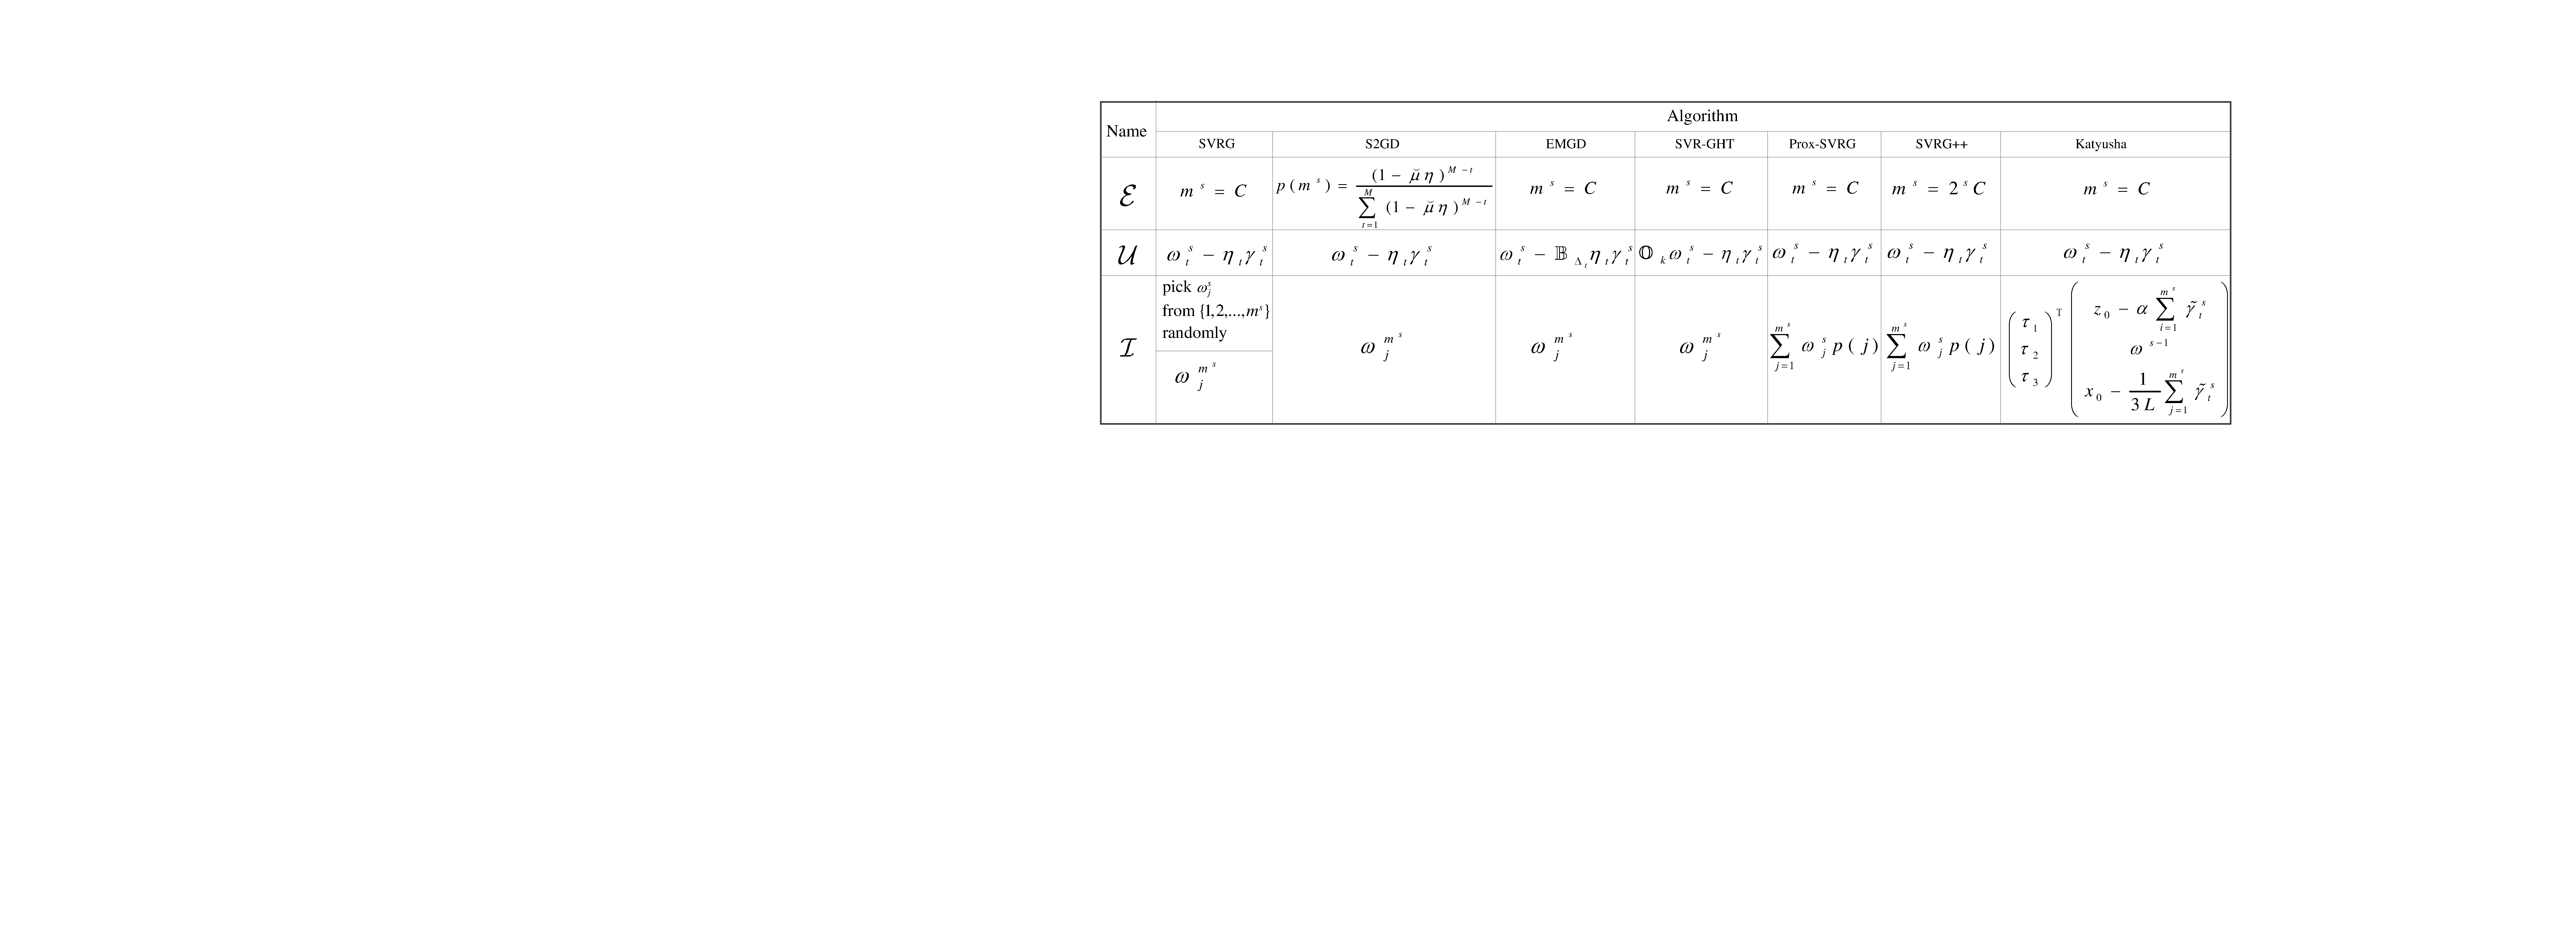
\includegraphics[width=2\columnwidth]{eui}}
\caption{Many existing variants of SGD with the variance reduction technique can be described by the general framework EUI.}
\label{figure_EUI_example}
\end{figure*}



\subsection{The analysis of the variance}
\label{subsect_variance_analysis}
It is obvious that the research about the variance reduction technique is really active. Not limited in the Fig. \ref{figure_EUI_example},  there exist various variants of SGD which using the variance reduction technique. But they usually adopts the same reduced variance stochastic gradient, i.e. Equ. \ref{equa_variance_metric_vr}, to update the parameter. We take SVRG  as an example to analyse the improvement of other following work.

As illustrated in Equ. \ref{equa_variance_metric_vr}, the first item of $v_t$ is the stochastic gradient which is denoted by the "variance source". The second item of $v_t$ is denoted by the "variance reducer" which is used to reduce the variance. The third item of $v_t$ is denoted by the " progressive direction" which makes sure that $v_t$ will not be too far away from the full gradient when updating parameter in an epoch. To better understand the potential of the variance reduction technique, we illustrate another two situations i.e. SGD and GD whose update gradient are denoted by $\gamma_t^{\text{SGD}}$ and $\label{equa_variance_metric_gd}
\gamma_t^{\text{GD}}$, respectively.  As illustrated in Equ. \ref{equa_variance_metric_sgd}, the variance of SGD is not reduced, and we refer its variance to the maximum. On the contrary, as illustrated in Equ. \ref{equa_variance_metric_gd}, the update gradient GD will not lead to the variance, and we thus refer the variance of GD as the minimum. 

\begin{equation}
\label{equa_variance_metric_sgd}
 \gamma_t^{\text{SGD}}=\nabla f_{i_t}(\omega_{i_t}^s)-\frac{1}{n}\sum\limits_{i=1}^n\nabla f_i(\tilde{\omega}^s)+\frac{1}{n}\sum\limits_{i=1}^n\nabla f_i(\tilde{\omega}^s);
\end{equation}
\begin{equation}
\label{equa_variance_metric_vr}
\gamma_t=\nabla f_{i_t}(\omega_{i_t}^s)-\nabla f_{i_t}(\tilde{\omega}^s)+\frac{1}{n}\sum\limits_{i=1}^n\nabla f_i(\tilde{\omega}^s);
\end{equation}
\begin{equation}
\label{equa_variance_metric_gd}
\gamma_t^{\text{GD}}=\nabla f_{i_t}(\omega_{i_t}^s)-\nabla f_{i_t}(\omega_{i_t}^t)+\frac{1}{n}\sum\limits_{i=1}^n\nabla f_i(\tilde{\omega}^s);
\end{equation}

It is obvious that the difference among the update gradients of SGD, GD and the variance reduction technique is the variance reducer. SGD has the maximal variance because its variance reducer  is a constant which does not help to reduce the variance. GD has no variance because that its variance reducer reduce all the variance caused by the variance source. The variance reducer of the variance reduction technique is a tradeoff between those of SGD and GD, which consists of a constant input parameter, i.e. $\tilde{\omega}^s$ and a stochastic gradient, i.e. $\nabla f_{i_t}(\cdot)$. It does not reduce all the variance like that of GD because that the constant input parameter, i.e. $\tilde{\omega}^s$ is stale for the iterations in an epoch. In specific, the staleness of $\tilde{\omega}^s$ against $\omega_{i_t}^s$ causes the variance during the update in an epoch. Therefore, the variance caused by the stale parameter in the variance reducer will be accumulated with the iterative updates in an epoch.  
Such the staleness of the parameter can be measured by  the distance $d_t$ between $\omega_{i_t}^s$ and $\tilde{\omega}^s$ with $d_t = \parallel \omega_{i_t}^s - \tilde{\omega}^s \parallel^2$. $d_0 = \parallel \omega_{i_0}-\tilde{\omega}^s\parallel^2 = 0$ according to the framework. Therefore, we obtain Theorem \ref{theorem_vr_lower_bound} as follows.


\newtheorem{Theorem}{\bf{Theorem}}
\newtheorem{Lemma}{\bf{Lemma}}



\begin{Theorem}
\label{theorem_vr_lower_bound}
If $\gamma_t$ is $p$-dimensional, and can be denoted by  $\gamma_t = (a_t^1, a_t^2..., a_t^p)$.   After $t$ iterations in the epoch, the distance $d_t$ holds that $d_t \ge p \eta^2\sum\limits_{j=1}^t a_j^2$ when the learning rate, i.e. $\eta_j$ with $j=1,2, ...m^s$ is a constant.
\end{Theorem}

As demonstrated in Theorem \ref{theorem_vr_lower_bound}, the distance becomes large with a large learning rate $\eta$, a high dimension $p$, and the increase of the number of the iterations in an epoch, i.e. $m^s$. Given a specific optimisation objective where $p$ is determined, if a constant learning rate is adopted, the variance is controlled by the design of the epoch size $m^s$ and the average of the element of every dimension  in the update gradient, i.e.  $\frac{1}{p}\sum\limits_{i=1}^p a_j^i$.  Therefore,  when the optimisation objective is determined, the variance is impacted by three aspects: the epoch size, the update rule and the parameter identification for the next iteration.

 As illustrated in \ref{figure_EUI_example}, the epoch size, i.e. $m^s$ is designed as a constant in EMGD, SVR-GHT, Prox-SVRG, Katyusha, and designed as an ascending variable for SVRG++ and S2GD. It is noting that the design of an appropriate epoch size is not trivial. A large size of an epoch causes much variance due to the large distance according to Theorem \ref{theorem_vr_lower_bound}. However, a small epoch size means that more epochs are required to keep the loss function converge within a given bound. Since the full gradient is required to be computed in an epoch, a large amount of epochs  thus lead to many gradient calculations which are very time-consuming.  

The update rule has an impact on the variance via $a_j^i$ according to Theorem \ref{theorem_vr_lower_bound}. Most variants of reduced variance SGD including S2GD, Prox-SVRG, SVRG++, and Katyusha adopt the same update rule with SVRG. EMGD updates the parameter within a bound in the high dimensional space. The bound is decaying so that the value of parameters will not be changed sharply, which decreases the variance. SVR-GHT introduces a hard-thresholding mechanism. Such the mechanism keeps the $k$ largest entries in the parameter, and sets other entries to zero when updating the parameter. Since SVR-GHT is designed for a class of optimisation objective where the optimal parameter has at most $k$ non-zero values,  the value of $a_j^i$ for an iteration in an epoch is thus not large for an iteration.

The identification of the parameters is to provide the initial parameters, i.e. $\omega^{s+1}$ for the next epoch. The variance in the current epoch will be introduced to the next epoch via the underlying identification of the parameter. Generally, the identification of the parameter is a tradeoff between the updates and the variance. First, we would like to use the updates which are obtained in the current epoch to train the parameters in the next epoch because those updates of the parameter help converge the loss function. Second, the variance existing in those updates is harmful to the convergence of the loss function. The more updates we use, the more variance may be introduced in the next epoch. As illustrated in Fig. \ref{figure_EUI_example}, most of the previous work uses $\tilde{\omega}_t^s$ as the initial parameter of the next epoch, which contains all the updates of the current epoch. Prox-SVRG and SVRG++ use the average of the sequence of the parameters, i.e. $\frac{1}{m^s}\sum\limits_{t=1}^{m^s}\omega_t^s$ which leads to less variance for the initial parameter of the next epoch, but disgards some updates of the parameter in the current epoch. 



\section{EstimateVR: a new reduced variance SGD}
\label{sect_estimate_vr}

\begin{algorithm}[t]
    \caption{EstimateVR}
    \label{algorithm_estimatevr}
    \begin{algorithmic}[1]
        \Require $\omega^0\in \mathbb{R}^d$. $\forall i\in[n]$, and $[n]$ represents $\{1,2, ..., n\}$. $\phi=0.001$, $\alpha=0.025$, $k^0=n$, and $g^0=0$.
        \State $P(i_t)\leftarrow \frac{1}{n}$ where $i_t \in \{1,2, ..., n\}$. $t$ is a positive integer;
        \For {$s=0,1,2,...,S$}
            \State $\omega_0^s=\tilde{\omega}^s$;
            \For {$t=0,1, ..., m-1$}
                \State  $v=\nabla f_{i_t}(\omega_t^s)-\nabla f_{i_t}(\tilde{\omega}^s)$;
                \State $\gamma_{t+1}^s=v+g^s$;
                \State $\omega_{t+1}^s = \omega_t^s - \eta \gamma_{t+1}^s$;
            \EndFor
            \State $\tilde{\omega}^{s+1} = \omega_m^s$;
            \State $\tilde{\gamma}=\textbf{estimateFullGradient}([\omega_{1:m}^{s}], \epsilon)$;
              \State $g^{s+1} = \tilde{\gamma}$;
          \EndFor
        \Return $\tilde{\omega}^S$.
    \end{algorithmic}
\end{algorithm}

Although  the variance reduction technique is effective to decrease the variance caused by the stochastic gradient, it has to keep a snapshot of the full gradient for every epoch. Unfortunately, the computation of the full gradient contains extensive gradient calculations which  are extremely time-consuming.  We design a new reduced variance SGD by using an estimate of the full gradient replacing the real computation of the full gradient to avoid the time-consuming gradient calculations. 

As illustrated in Algo. \ref{algorithm_estimatevr}, the new variant of SGD with the variance reduction technique is denoted by \emph{EstimateVR}. EstimateVR provides an interface denoted by \emph{estimateFullGrdient} which is used to implement the estimation of the full gradient. As illustrated in Fig. \ref{figure_estimate_full_gradient}, we provide two implementations to estimate the full gradient which are denoted by \emph{sampleVR} and \emph{reuseVR}, respectively. \emph{sampleVR} estimates the full gradient by using a subset of the instances; while \emph{reuseVR} estimates the full gradient by using the average of the stale parameters during the current epoch. 

\begin{figure}
\centering
\subfigure{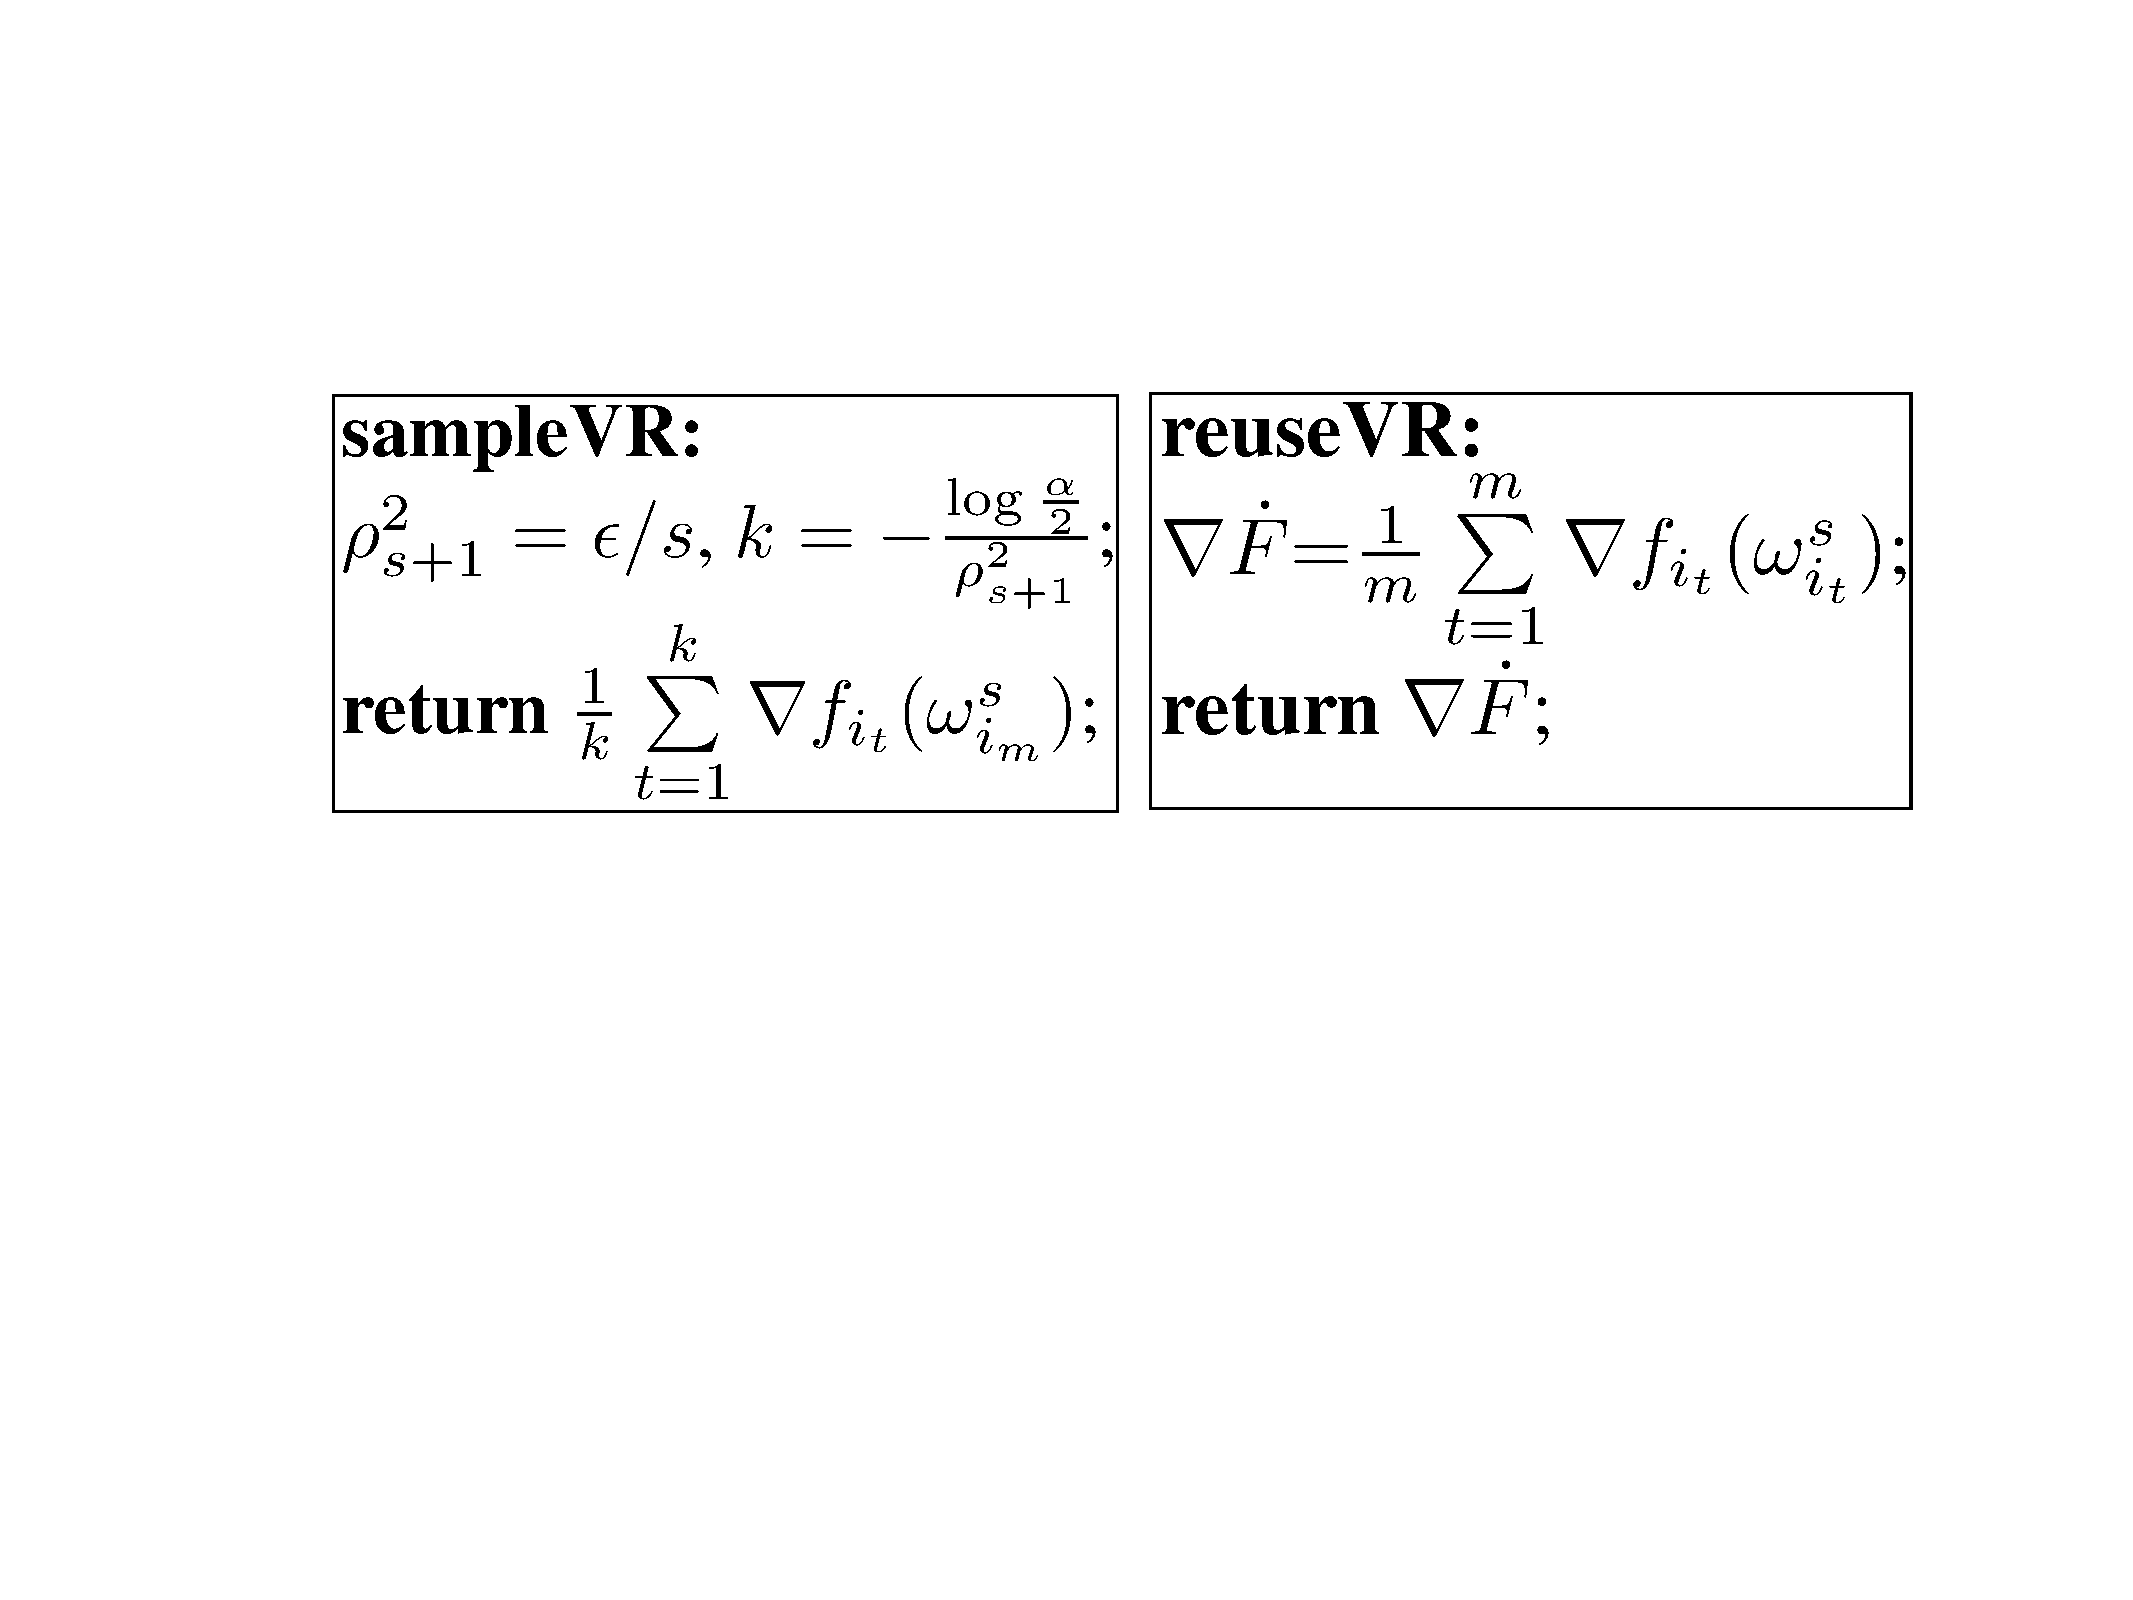
\includegraphics[width=0.8\columnwidth]{estimateFullGradient}}
\caption{The function \emph{estimateFullGradient} in Algo. \ref{algorithm_estimatevr} is presented with two implementations: \emph{sampleVR} and \emph{reuseVR}.}
\label{figure_estimate_full_gradient}
\end{figure}

\begin {itemize}
\item{sampleVR:} As illustrated in Equ. \ref{equ_estimate_vr_update_rule}, the $k$ instances are sampled from the training data, and we obtain the $k$ stochastic gradients. The average of them, i.e. $\frac{1}{k}\sum\limits_{i=1}^k\nabla f_i(\tilde{\omega}^s)$ is used as the progressive direction for the next epoch. Since $\mathbb{E} \left(  \frac{1}{k}\sum\limits_{i=1}^k\nabla f_i(\tilde{\omega}^s) \right)=  \mathbb{E} \left (\frac{1}{n}\sum\limits_{i=1}^n\nabla f_i(\tilde{\omega}^s) \right)  =  \nabla F(\tilde{\omega}^s)$ holds, the new update gradient, i.e. $\dot{\gamma_t}$ is the same with $\gamma_t$ in probability, that is, $\mathbb{E} (  \dot{\gamma_t}) = \mathbb{E} (\gamma_t) = \nabla F(\omega_{i_t}^s)$. 
\begin{equation}
\label{equ_estimate_vr_update_rule}
\dot{\gamma_t}=\nabla f_{i_t}(\omega_{i_t}^s)-\nabla f_{i_t}(\tilde{\omega}^s)+\frac{1}{k}\sum\limits_{i=1}^k\nabla f_{i_k}(\tilde{\omega}^s);
\end{equation}
The estimate of the full gradient is denoted by $\dot{g} = \frac{1}{k}\sum\limits_{i=1}^k\nabla f_i(\tilde{\omega}^s)$. Let $d^s = \dot{g}-g=(d_1^s, d_2^s, ..., d_p^s)$. Considering each element in $d^s$, i.e. $d_i^s$ with $i\in\{ 1,2, ..., p  \}$, we obtain $P(d_i^s \ge \rho) \le e^{-2k\rho^2}$ when sampling $k$ instances from a large amount of the training data randomly. If $\alpha = p (d_i^s\notin [-\rho, \rho] ) \le e^{-2k\rho^2}$, then the least number of samples, i.e. $k$ should satisfy
\begin{equation}
\label{equ_estimate_samples_lower_bound}
k\ge - \frac{\log \frac{\alpha}{2}}{\rho^2}
\end{equation} according to Hoeffding's inequality so that we can acquire $(1-\alpha)$-confidence interval $[-\rho, \rho]$.

\item{reuseVR:} As illustrated in Equ. \ref{equ_reuse_vr}, the average of the stochastic gradients is used to estimate the full gradient for the next epoch. The variance between the real full gradient and the estimation, i.e. $\nabla \dot{F} =\frac{1}{m}\sum\limits_{t=0}^{m-1} \nabla f_{i_t}(\omega_{t}^s)$ becomes large with the increase of the epoch size $m$. An effective way to solve this problem is to estimate the full gradient by using the last $n$ stochastic gradients, i.e. $\nabla \dot{F} = \frac{1}{n}\sum\limits_{t=m-n}^{m-1} \nabla f_{i_t}(\omega_{t}^s)$. 
\begin{equation}
\label{equ_reuse_vr}
\dot{\gamma_t}=\nabla f_{i_t}(\omega_{i_t}^s)-\nabla f_{i_t}(\tilde{\omega}^s)+\frac{1}{m}\sum\limits_{t=0}^{m-1} \nabla f_{i_t}(\omega_{t}^s);
\end{equation}. Since the stochastic gradients are computed in the iterations of the current epoch, the estimation of the full gradient does not lead to any more calculations of the gradient.
\end{itemize}

Although both \emph{sampleVR} and \emph{reuseVR} outperform the previous work in the empirical study, we provide the theoretical analysis of the convergence and the gradient complexity for \emph{sampleVR}. Such those analysis for \emph{reuseVR} will be left as the future work. As illustrated in Theorem \ref{theorem_converge} and \ref{theorem_gradient_complexity}, \emph{sampleVR} converges at a linear rate, but the linear rate is  not the best when comparing with SVRG and other following work. However, its gradient complexity is extremely smaller than the previous work because $\alpha$ is usually very small, for example $0.01$. Therefore, \emph{sampleVR} converges fast, and gains the best convergence performance in the extensive empirical studies.


\begin{Theorem}
\label{theorem_converge}
Let  $\delta = \frac{4 L \eta^2 m^s}{ \eta(1-2\eta L) m^s  -  \frac{1}{\gamma}    }     <1$, and $d^s$ in the $s_{th}$ iteration be small enough, so that $d^s\le F(\tilde{\omega}^s)-F(\omega_\ast)$ holds. EstimateVR has the linear convergence rate: \\
$F(\tilde{\omega}^{s+1}) - F(\omega_\ast)  \le \frac{1+2L}{2L}\delta  [F(\tilde{\omega}^s)-F(\omega_\ast)]$. Specifically, $\mathbb{E}\parallel d^s\parallel^2 = 0$ always holds, we thus obtain
$\mathbb{E}(F(\tilde{\omega}^{s+1}) - F(\omega_\ast) ) \le  \delta \mathbb{E}( [F(\tilde{\omega}^s)-F(\omega_\ast)]  )$.
\end{Theorem}


\begin{Theorem}
\label{theorem_gradient_complexity}
Assume the objective needs $s$ epochs to achieve to the $\epsilon$, and then the gradient complexity is $(1-\alpha)\left( m-\frac{1}{6} \frac{\log\frac{\alpha}{2}}{\rho_0^2} s(s+1)(2s+1) \right) + \alpha n$ atomic gradient computation.
\end{Theorem}





\section{Performance evaluation}
\label{sect_performance_evaluation}


\begin{figure*}[t]
\centering
\subfigure[ijcnn1]{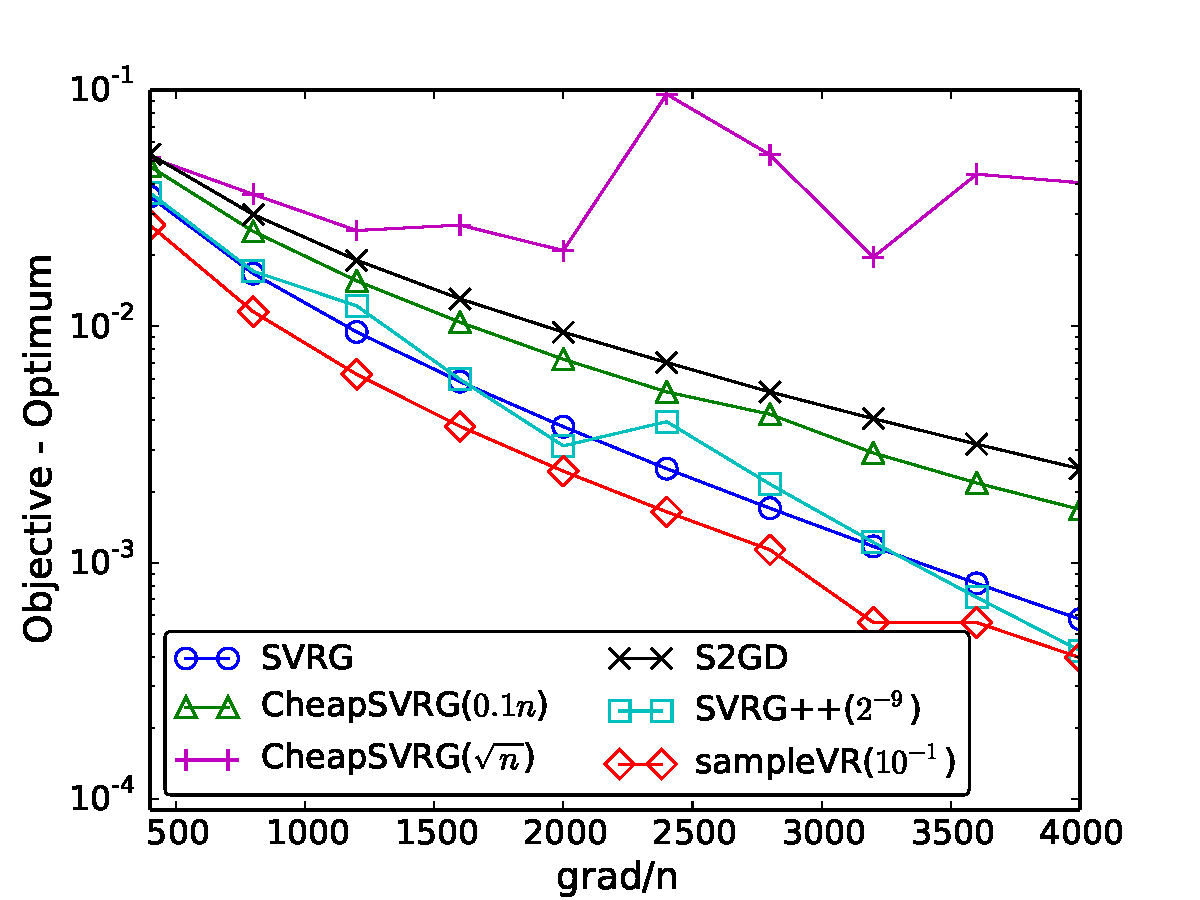
\includegraphics[width=0.5\columnwidth]{figure_ijcnn_convergence}\label{figure_ijcnn_convergence}}
\subfigure[colon-cancer]{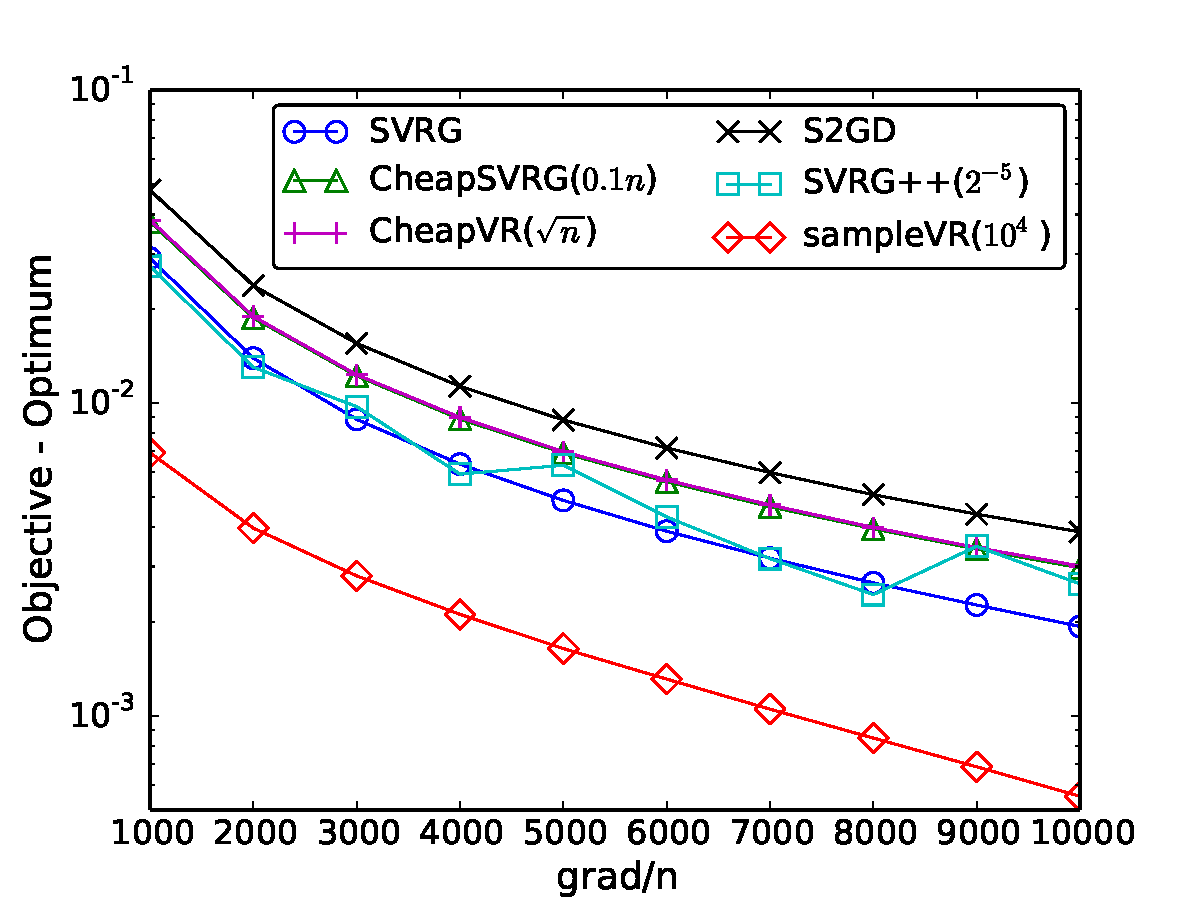
\includegraphics[width=0.5\columnwidth]{figure_colon-cancer_convergence}\label{figure_colon-cancer_convergence}}
\subfigure[duke-breast-cancer]{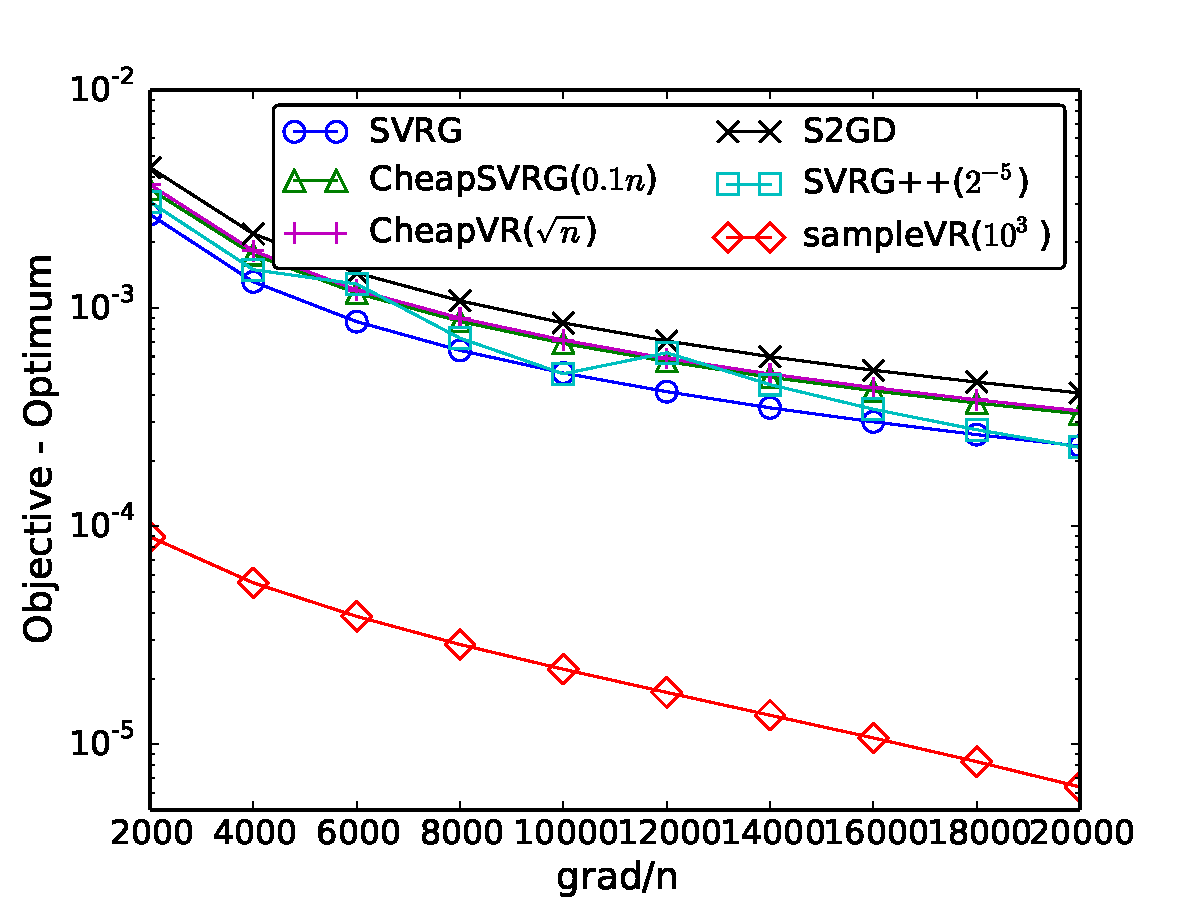
\includegraphics[width=0.5\columnwidth]{figure_duke_convergence}\label{figure_duke_convergence}}
\subfigure[a9a]{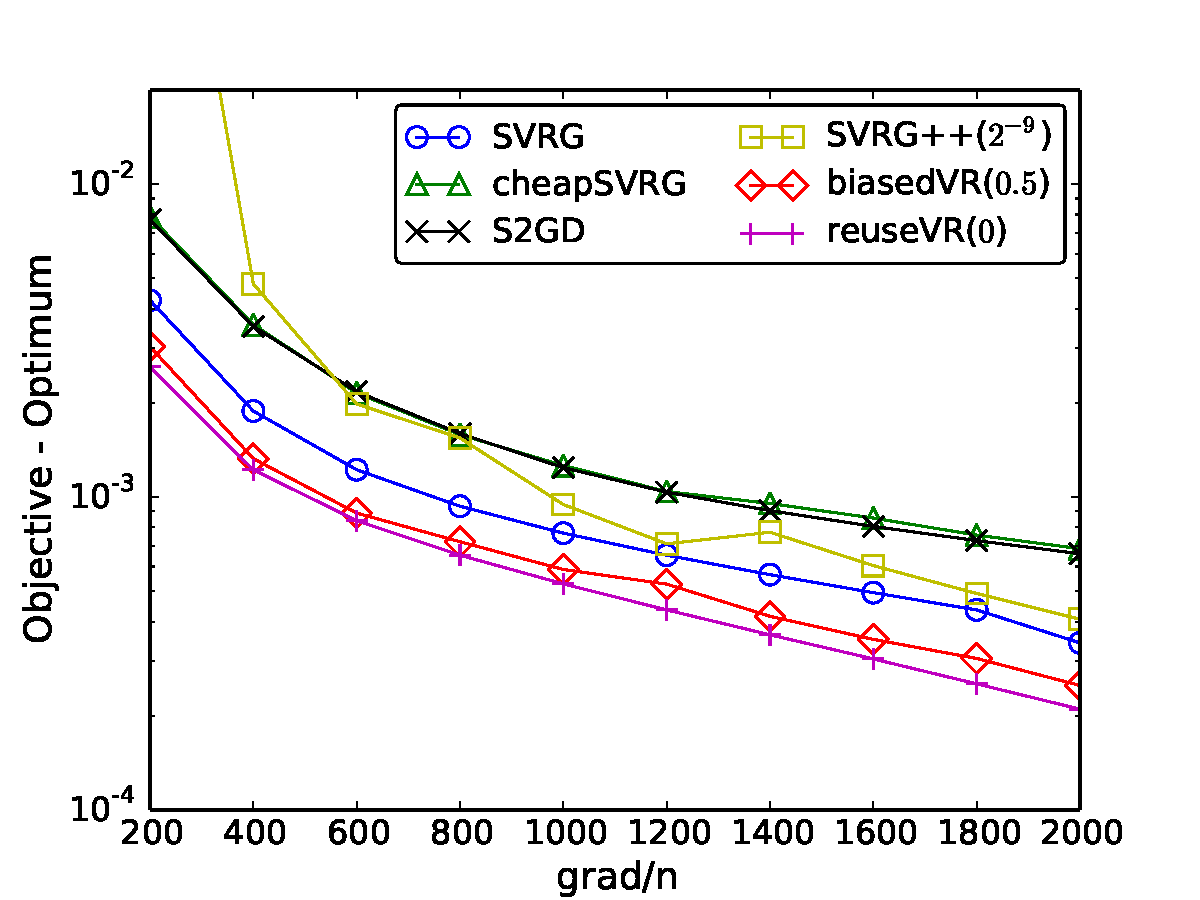
\includegraphics[width=0.5\columnwidth]{figure_a9a_convergence}\label{figure_a9a_convergence}}
\caption{Both \emph{sampleVR} and \emph{reuseVR} make the training loss of the $l2$-regularised logistic regression tasks converge faster than the other existing algorithms.}
\label{figure_logistic_regression_convergence}
\end{figure*}

\begin{figure*}[t]
\centering
\subfigure[ijcnn1]{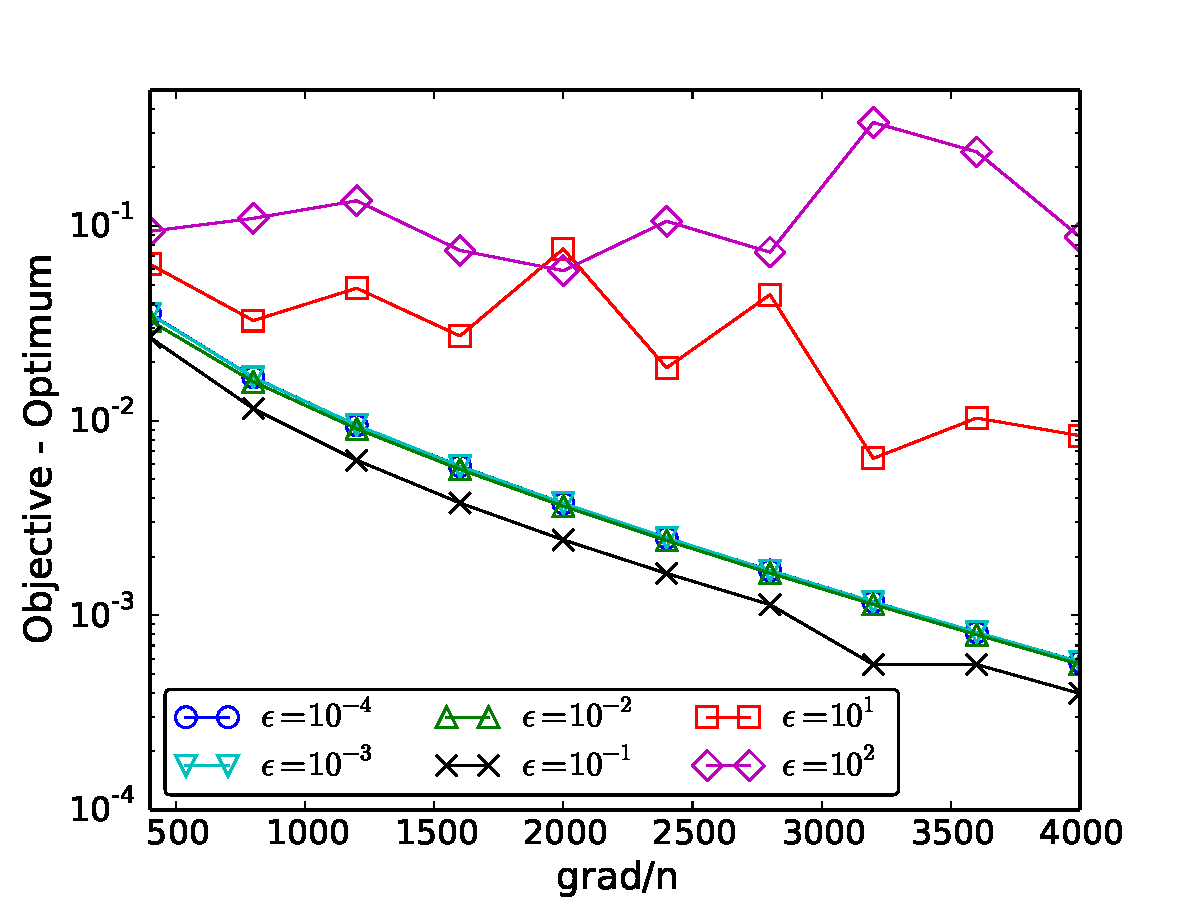
\includegraphics[width=0.5\columnwidth]{figure_ijcnn_rho}\label{figure_ijcnn_rho}}
\subfigure[colon-cancer]{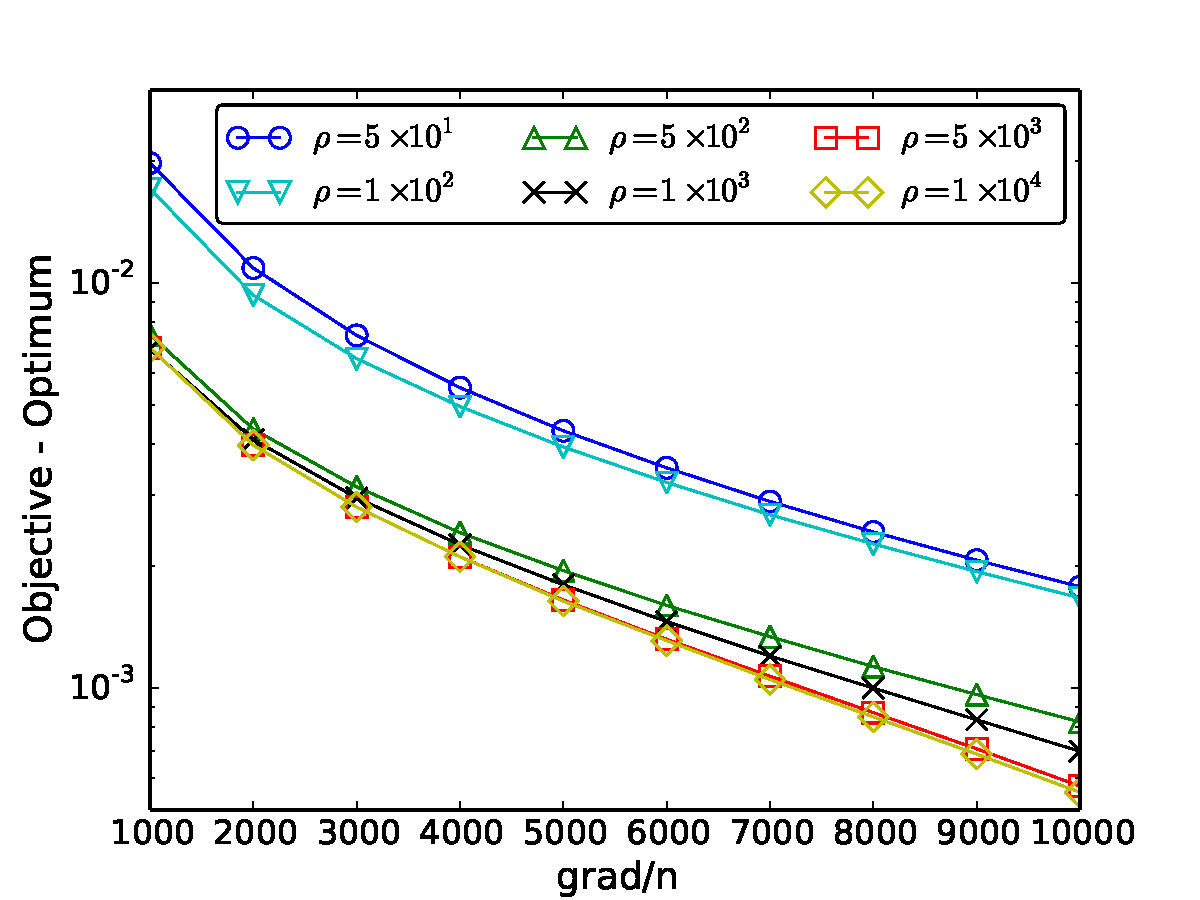
\includegraphics[width=0.5\columnwidth]{figure_colon-cancer_rho}\label{figure_colon-cancer_rho}}
\subfigure[duke-breast-cancer]{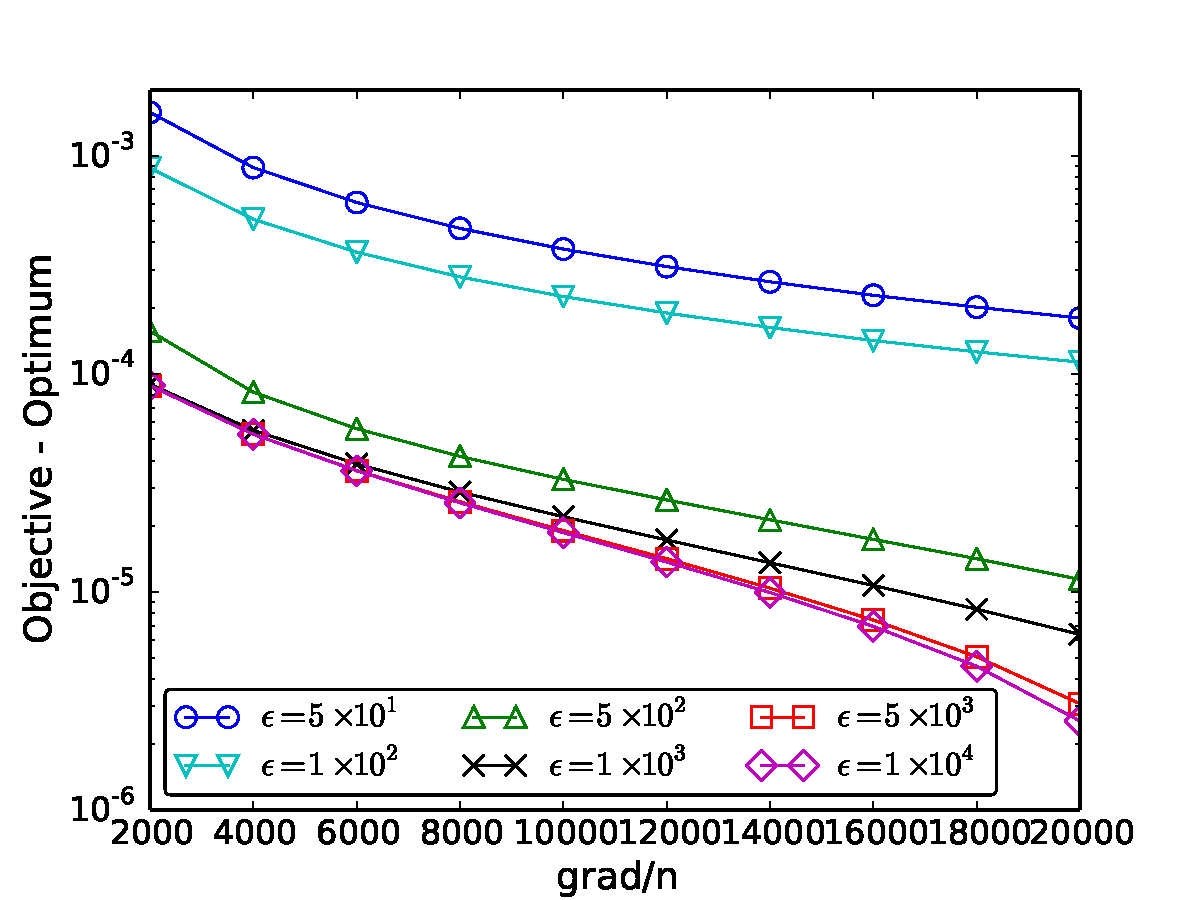
\includegraphics[width=0.5\columnwidth]{figure_duke_rho}\label{figure_duke_rho}}
\subfigure[a9a]{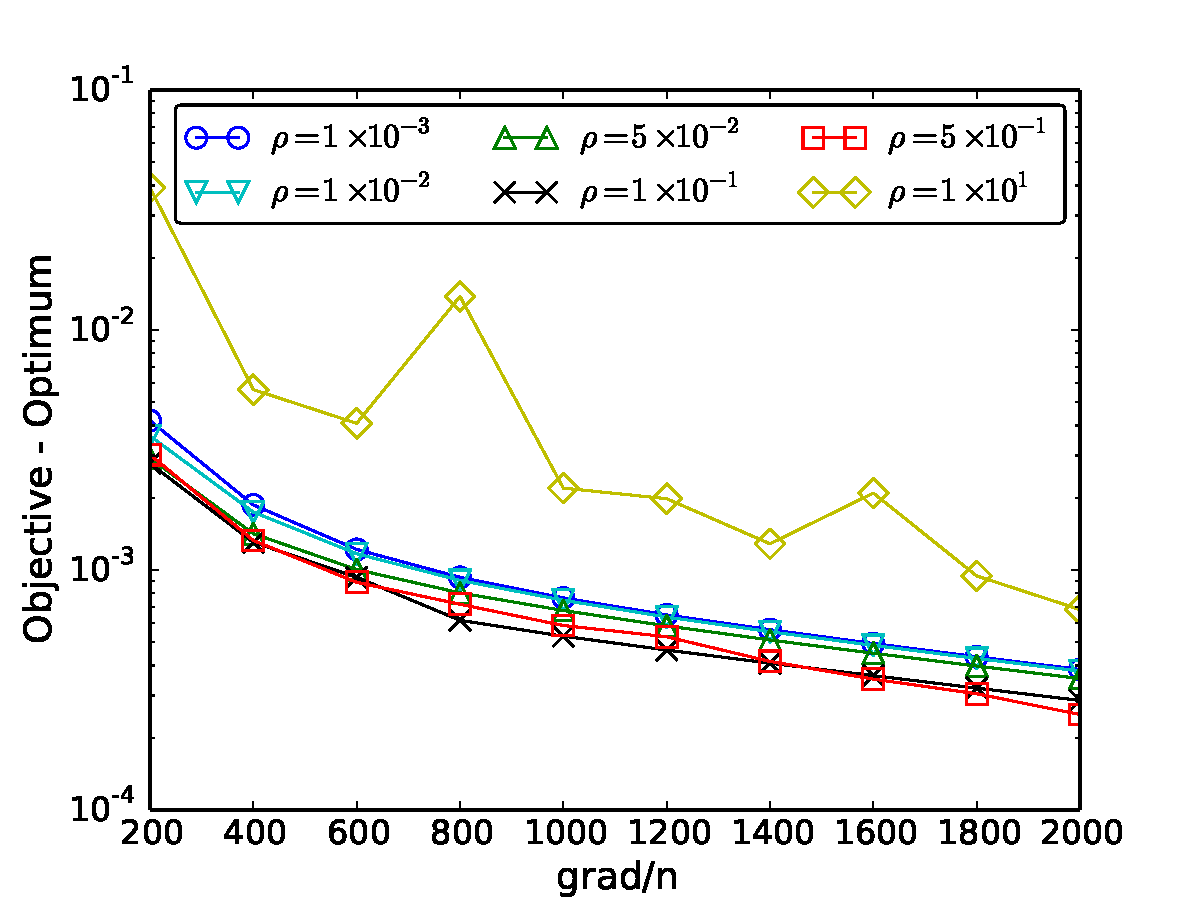
\includegraphics[width=0.5\columnwidth]{figure_a9a_rho}\label{figure_a9a_rho}}
\caption{Generally, \emph{sampleVR} with a large $\epsilon$ has a better performance for the the $l2$-regularised logistic regression tasks. However,  the increase of the variance with a too large $\epsilon$ slows the convergence of the training loss.}
\label{figure_logistic_regression_rho}
\end{figure*}

%\begin{figure*}[t]
%\centering
%\subfigure[ijcnn1]{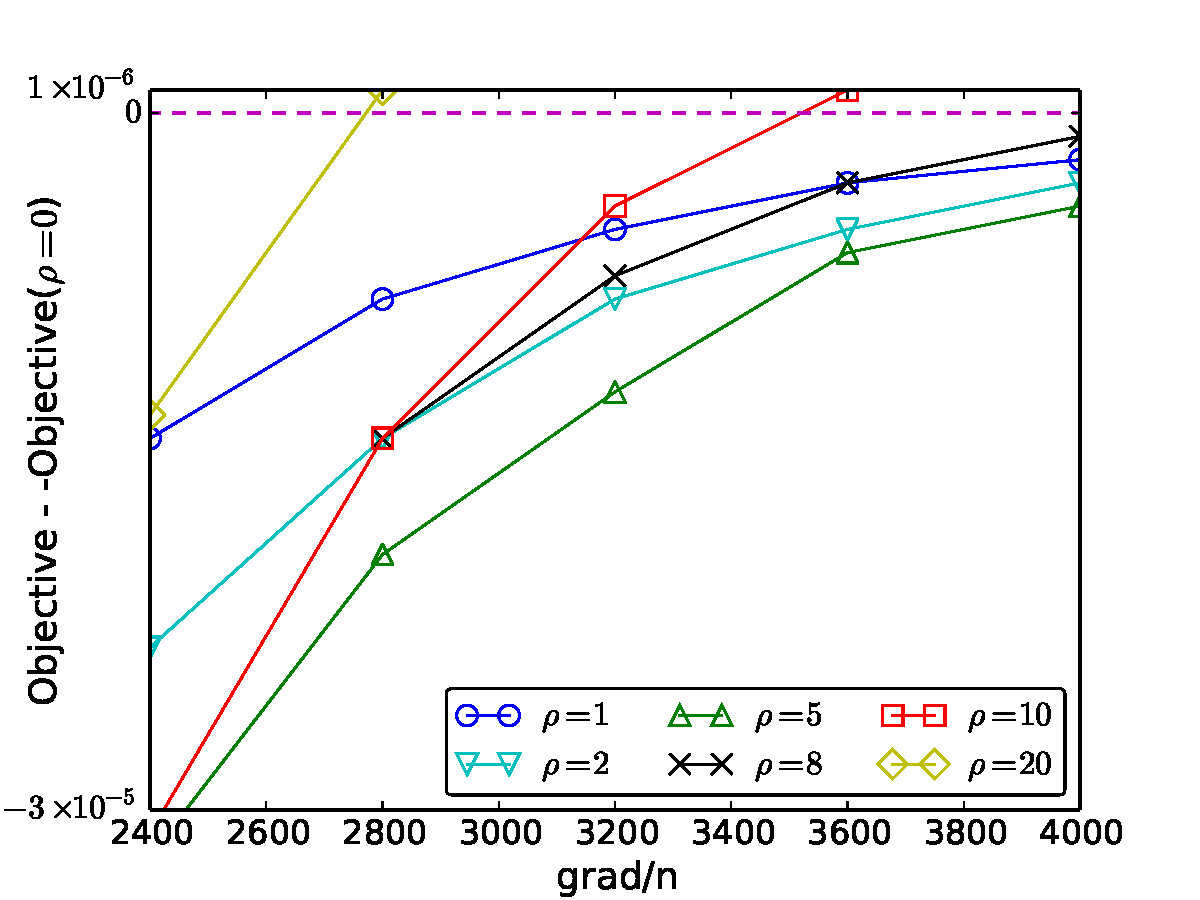
\includegraphics[width=0.5\columnwidth]{figure_ijcnn_rate}\label{figure_ijcnn_rate}}
%\subfigure[colon-cancer]{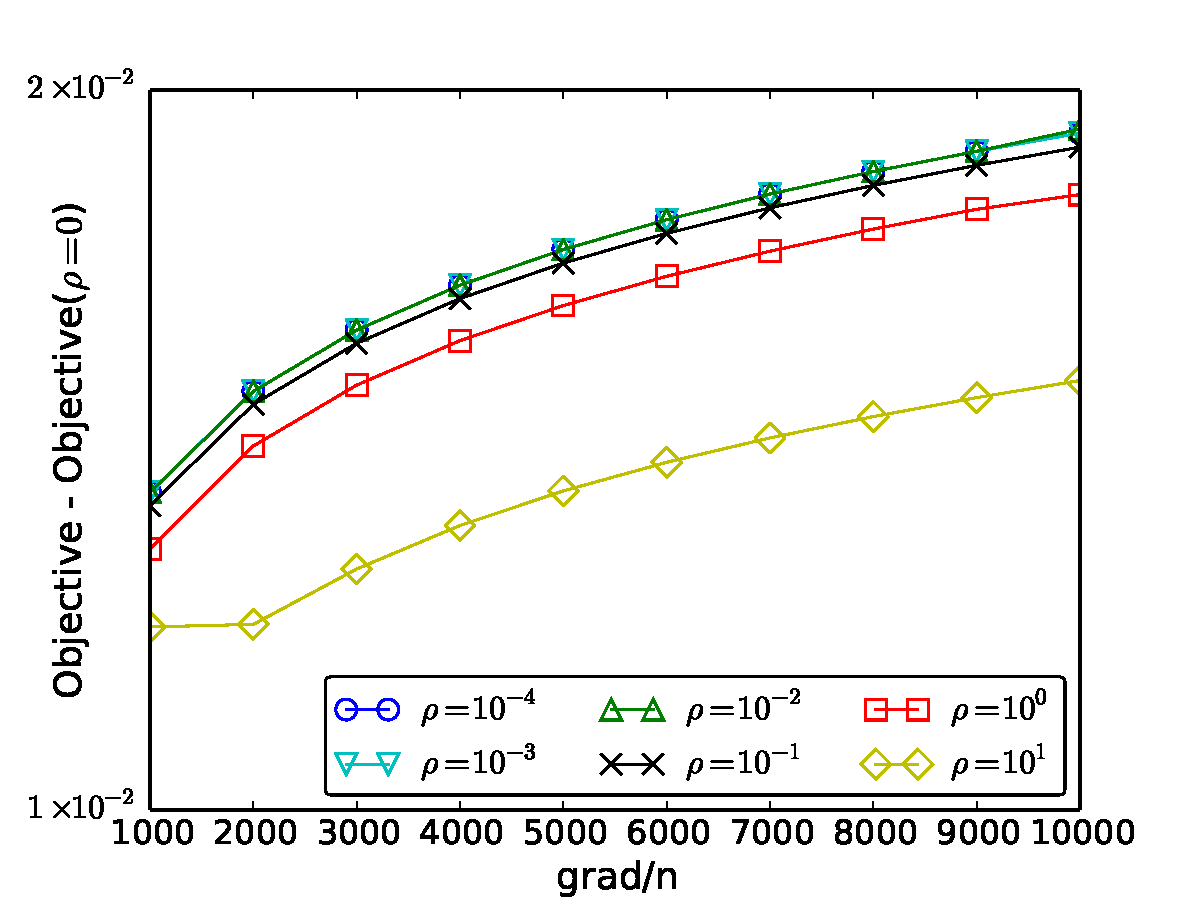
\includegraphics[width=0.5\columnwidth]{figure_colon-cancer_rate}\label{figure_colon-cancer_rate}}
%\subfigure[duke-breast-cancer]{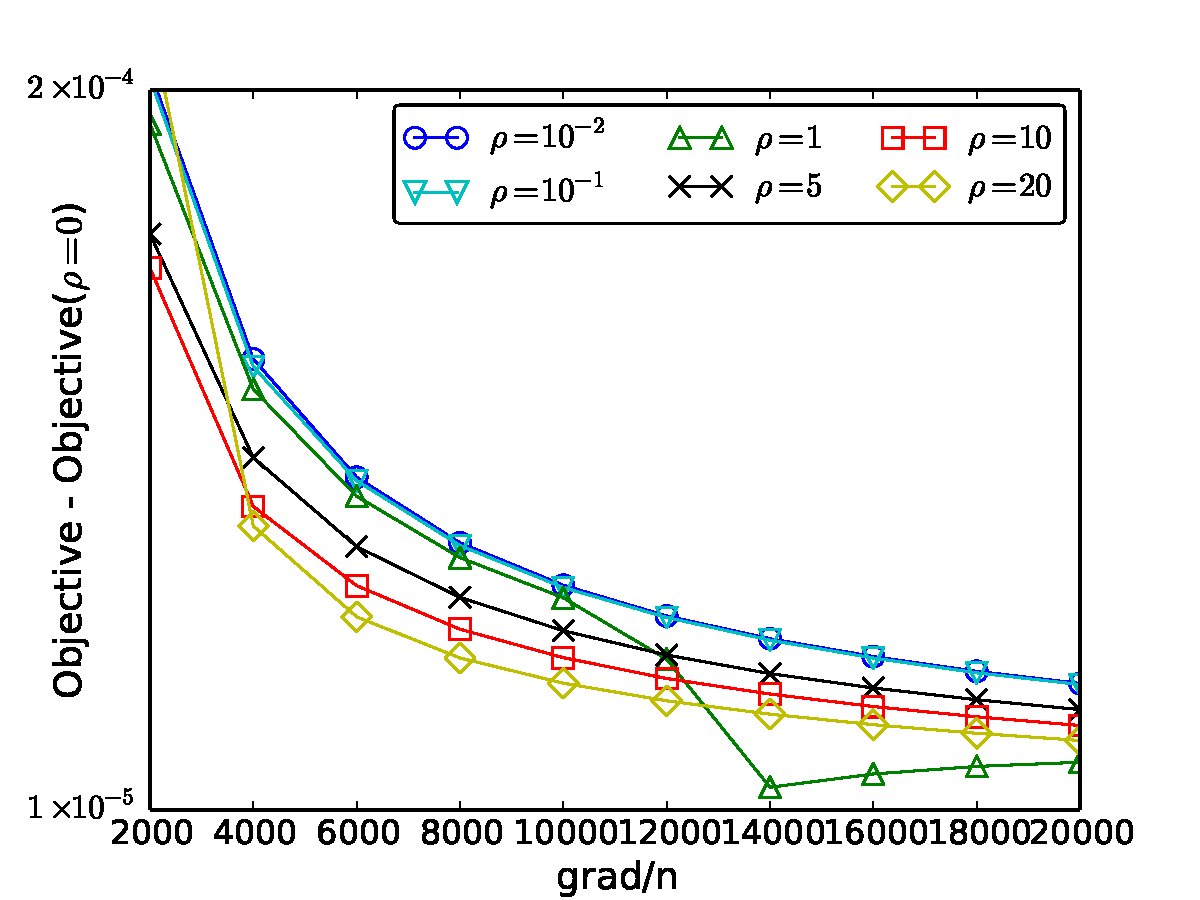
\includegraphics[width=0.5\columnwidth]{figure_duke_rate}\label{figure_duke_rate}}
%\subfigure[a9a]{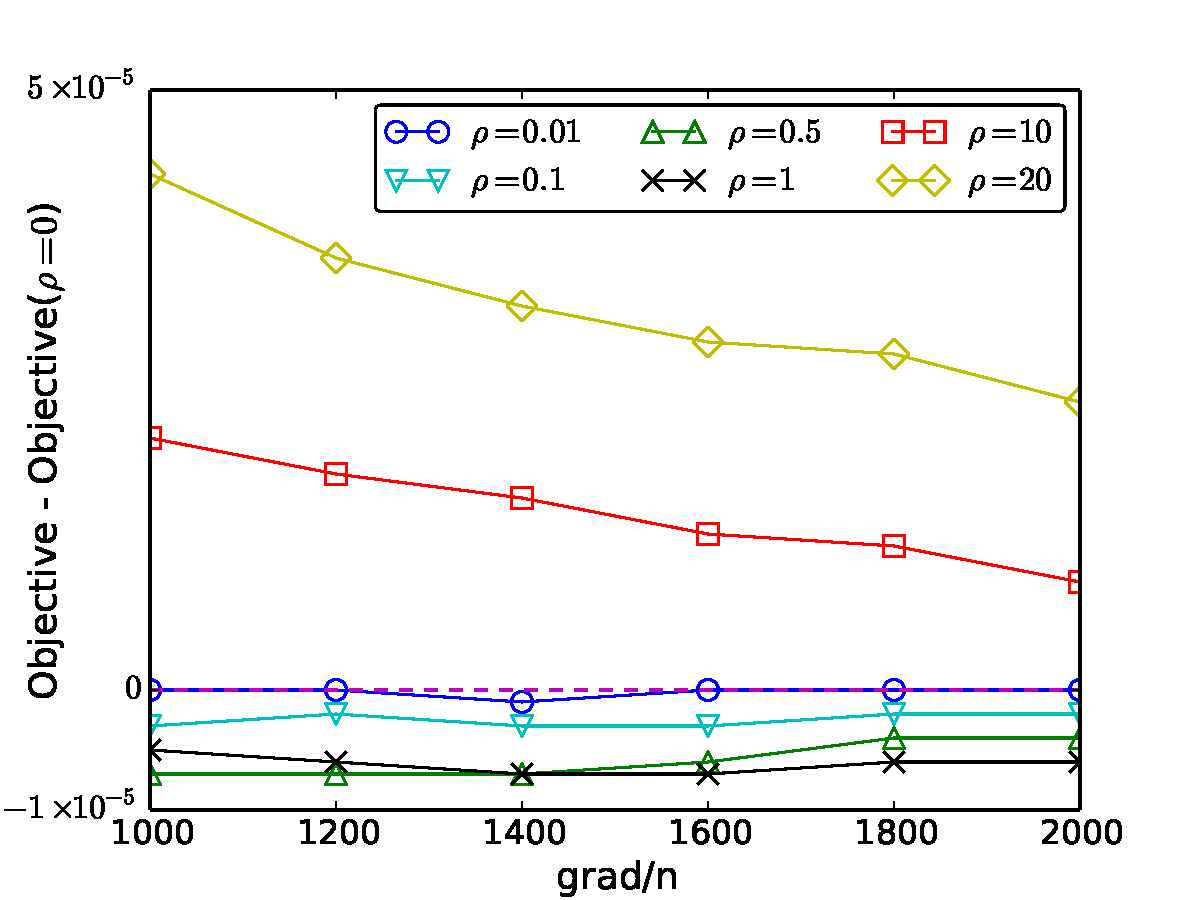
\includegraphics[width=0.5\columnwidth]{figure_a9a_rate}\label{figure_a9a_rate}}
%\caption{reuseVR}
%\label{figure_logistic_regression_rate}
%\end{figure*}



\begin{figure*}[t]
\centering
\subfigure[mg]{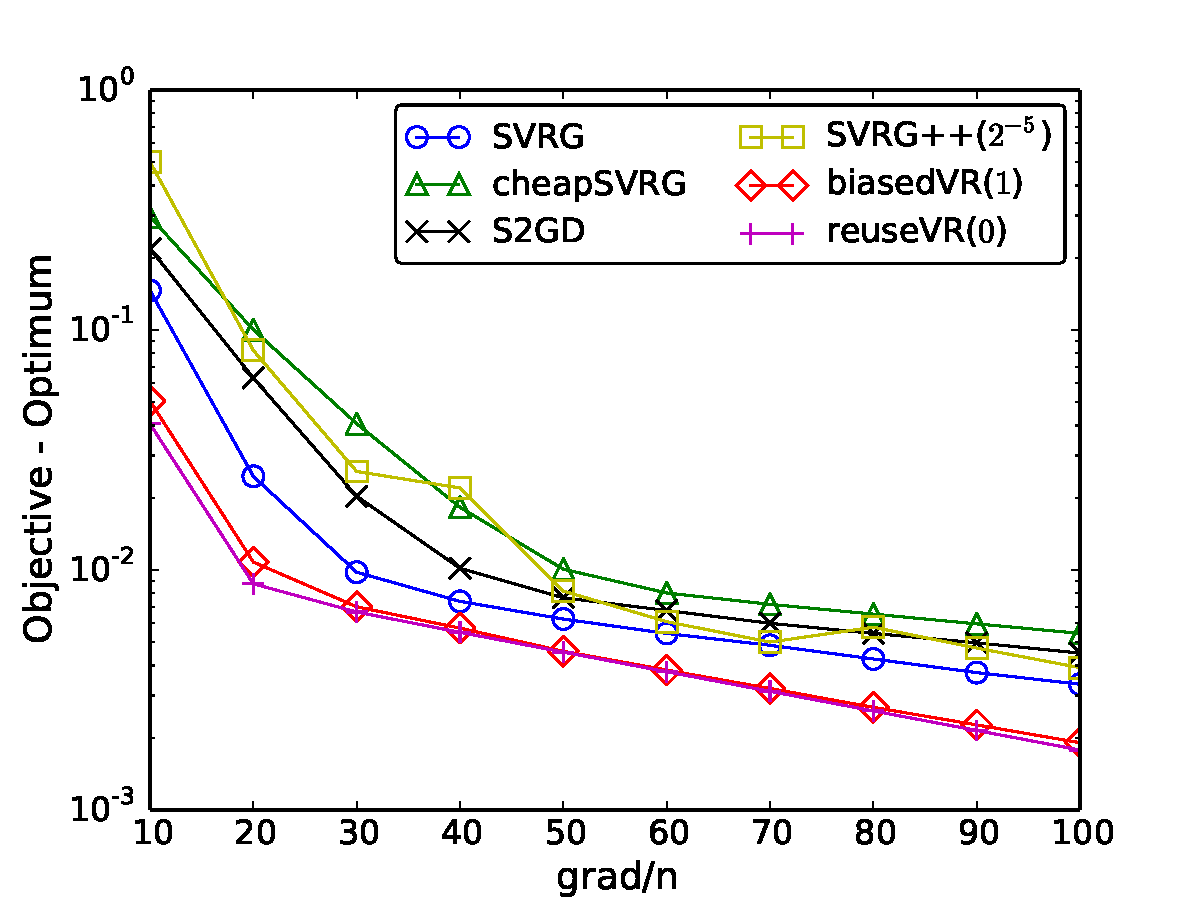
\includegraphics[width=0.5\columnwidth]{figure_mg_convergence}\label{figure_mg_convergence}}
\subfigure[cpusmall]{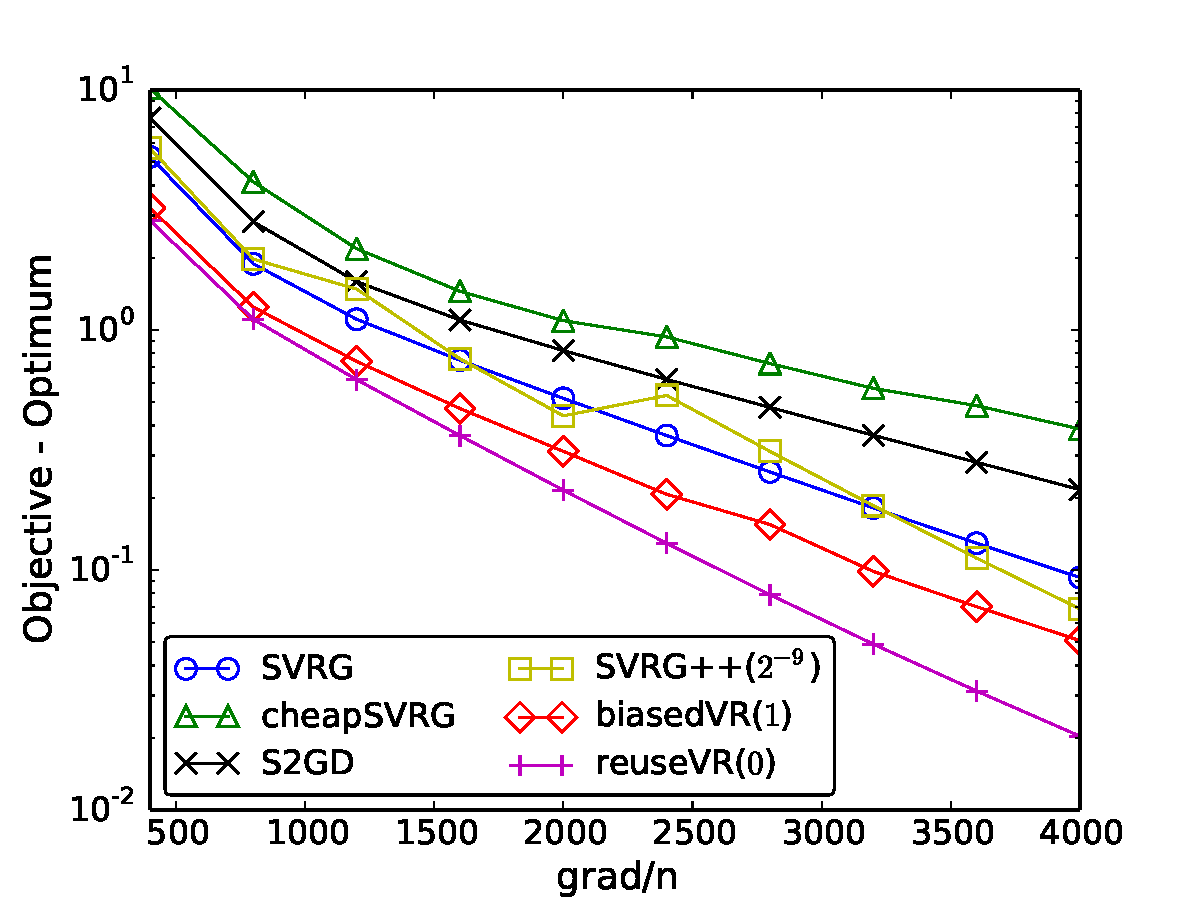
\includegraphics[width=0.5\columnwidth]{figure_cpusmall_convergence}\label{figure_cpusmall_convergence}}
\subfigure[yearPredictionMSD]{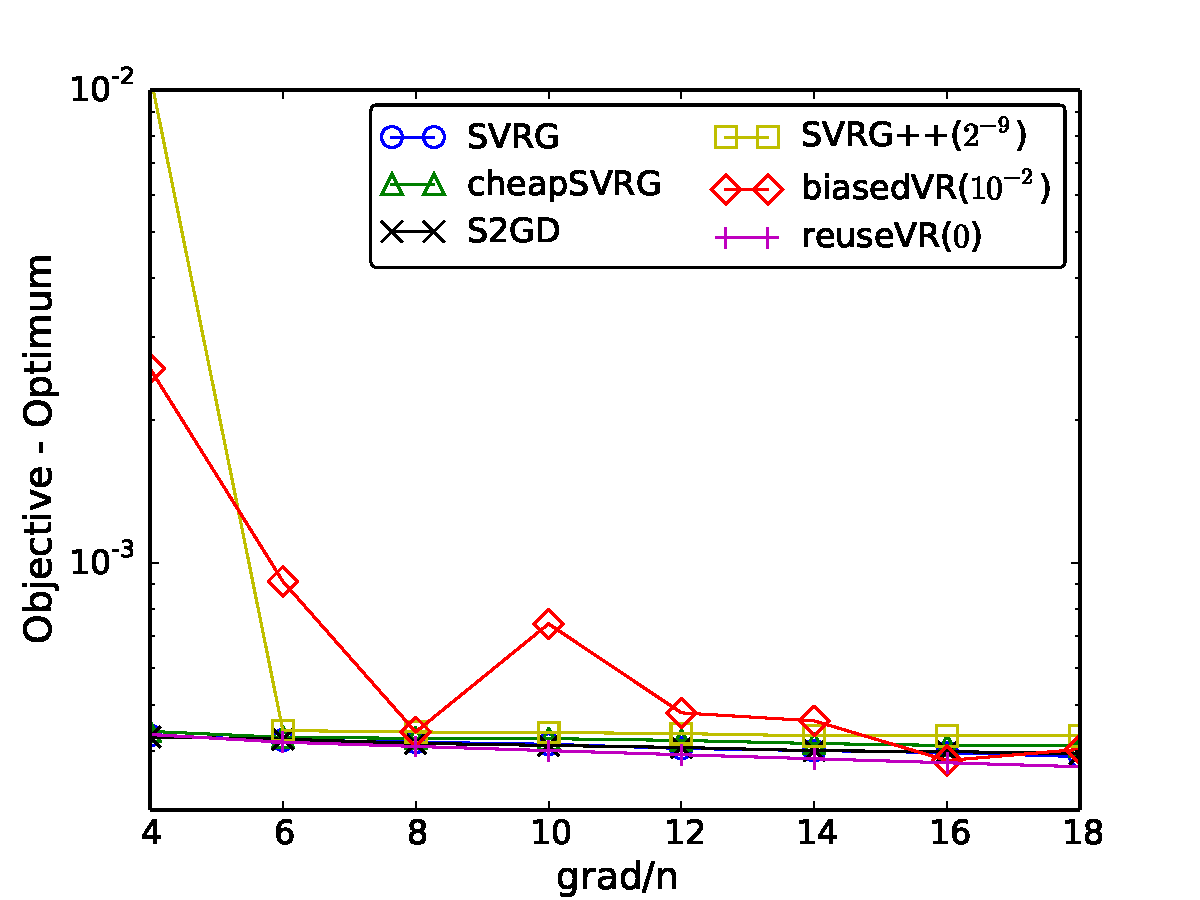
\includegraphics[width=0.5\columnwidth]{figure_year_convergence}\label{figure_year_convergence}}
\subfigure[space-ga]{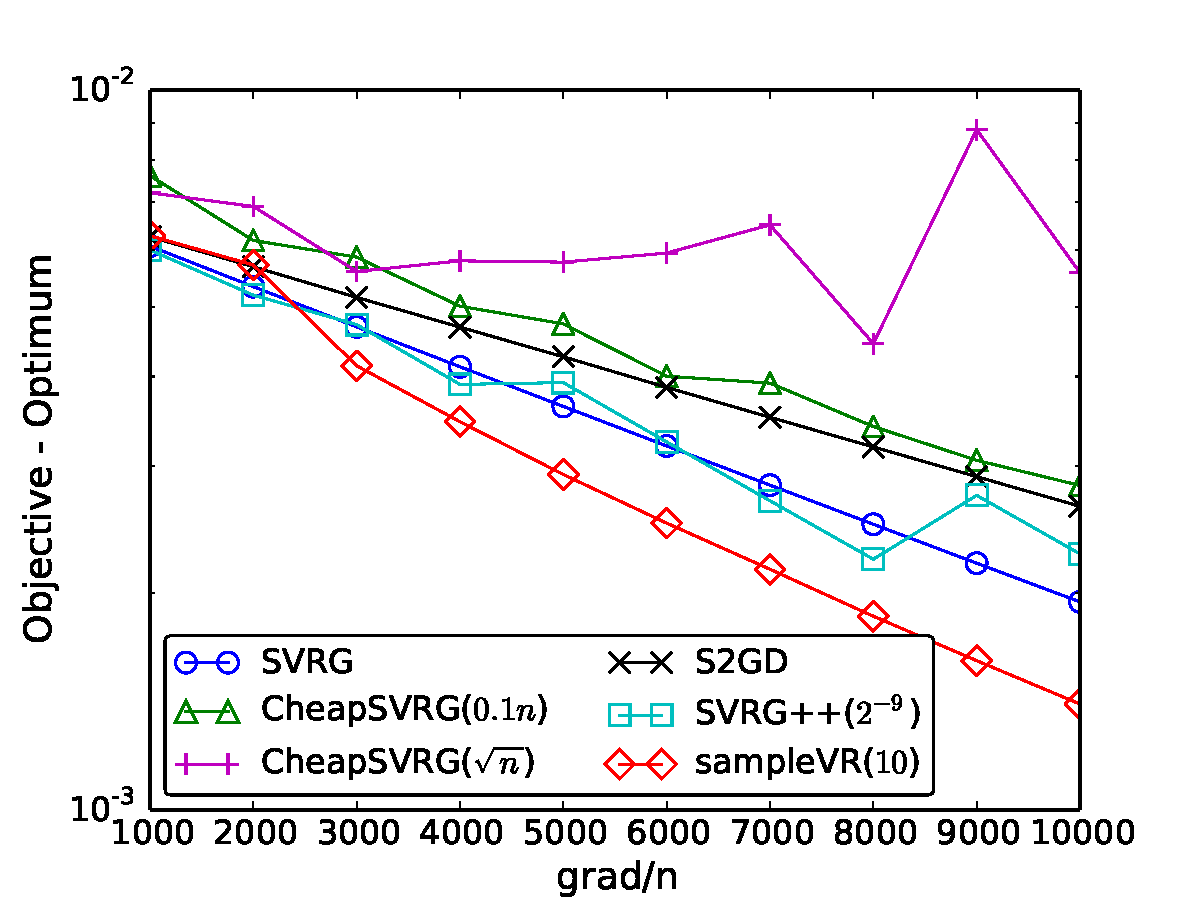
\includegraphics[width=0.5\columnwidth]{figure_space-ga_convergence}\label{figure_space-ga_convergence}}
\caption{Generally, both \emph{sampleVR} and \emph{reuseVR} outperforms the other existing algorithms on the convergence of the training loss when conducting the ridge regression tasks.}
\label{figure_ridge_regression_convergence}
\end{figure*}



\begin{figure*}[t]
\centering
\subfigure[mg]{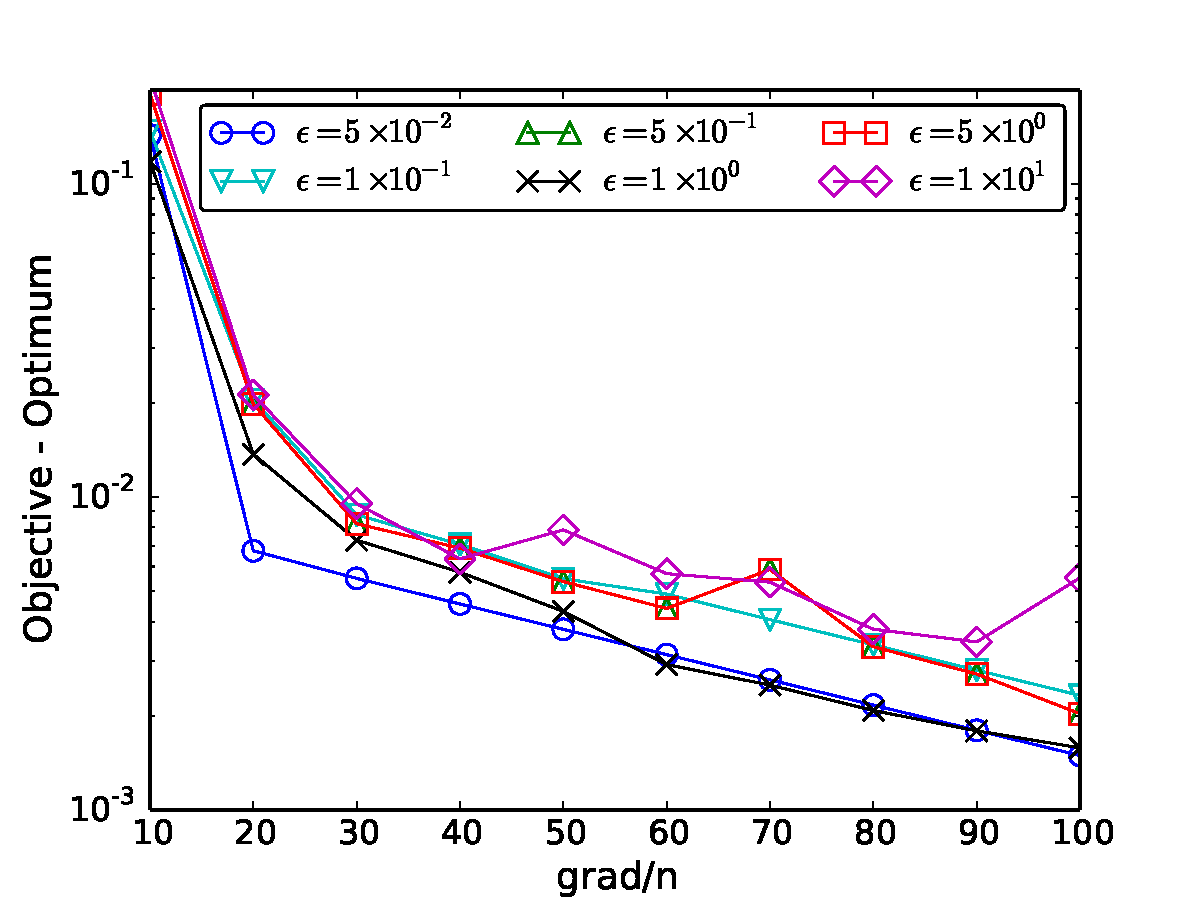
\includegraphics[width=0.5\columnwidth]{figure_mg_rho}\label{figure_mg_rho}}
\subfigure[cpusmall]{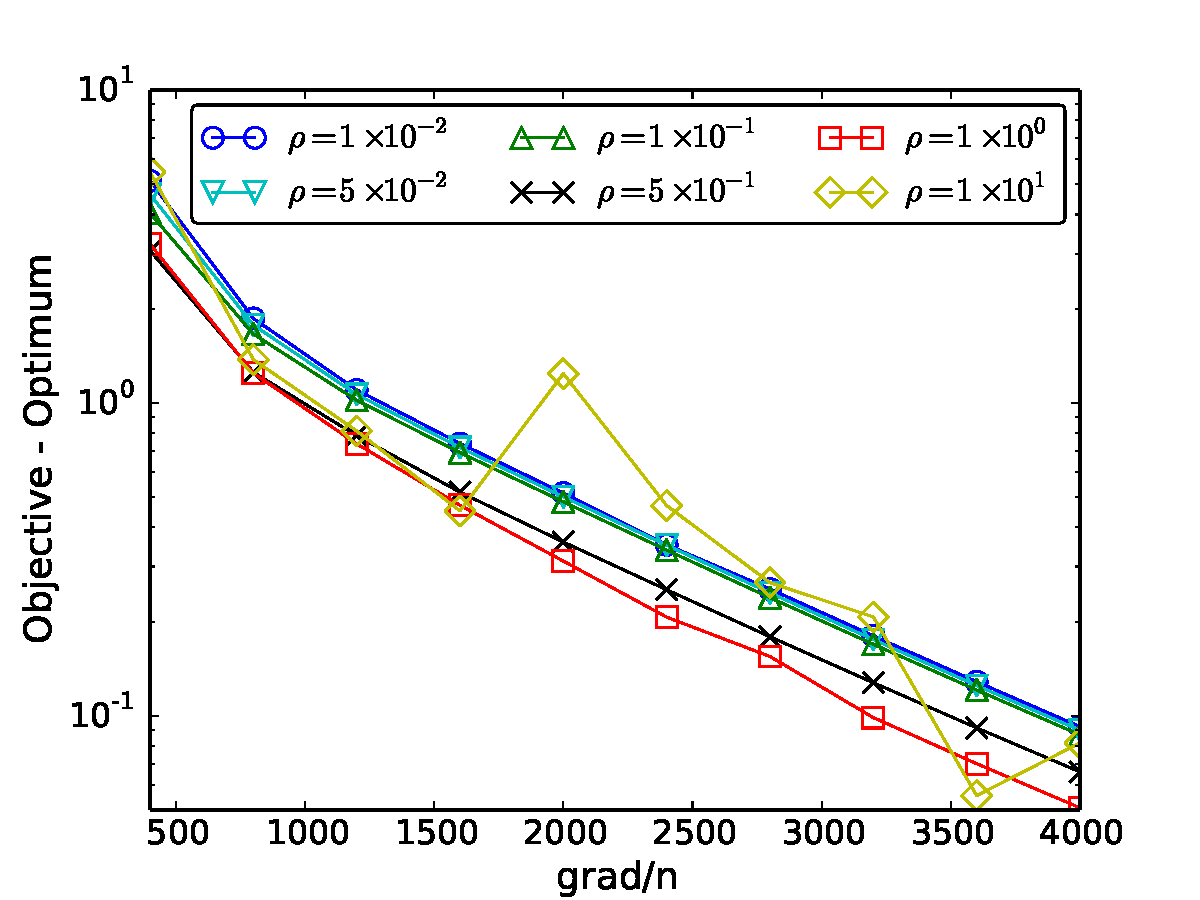
\includegraphics[width=0.5\columnwidth]{figure_cpusmall_rho}\label{figure_cpusmall_rho}}
\subfigure[yearPredictionMSD]{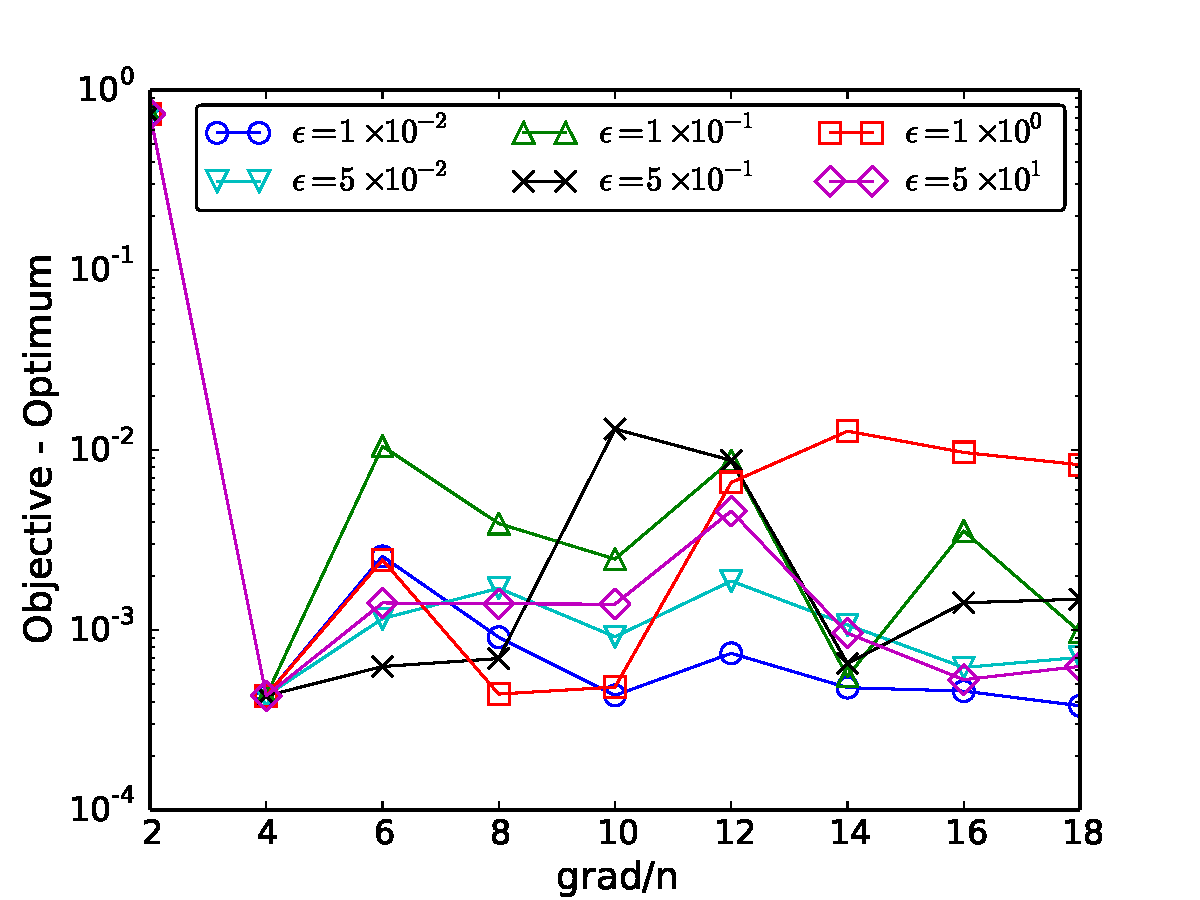
\includegraphics[width=0.5\columnwidth]{figure_year_rho}\label{figure_year_rho}}
\subfigure[space-ga]{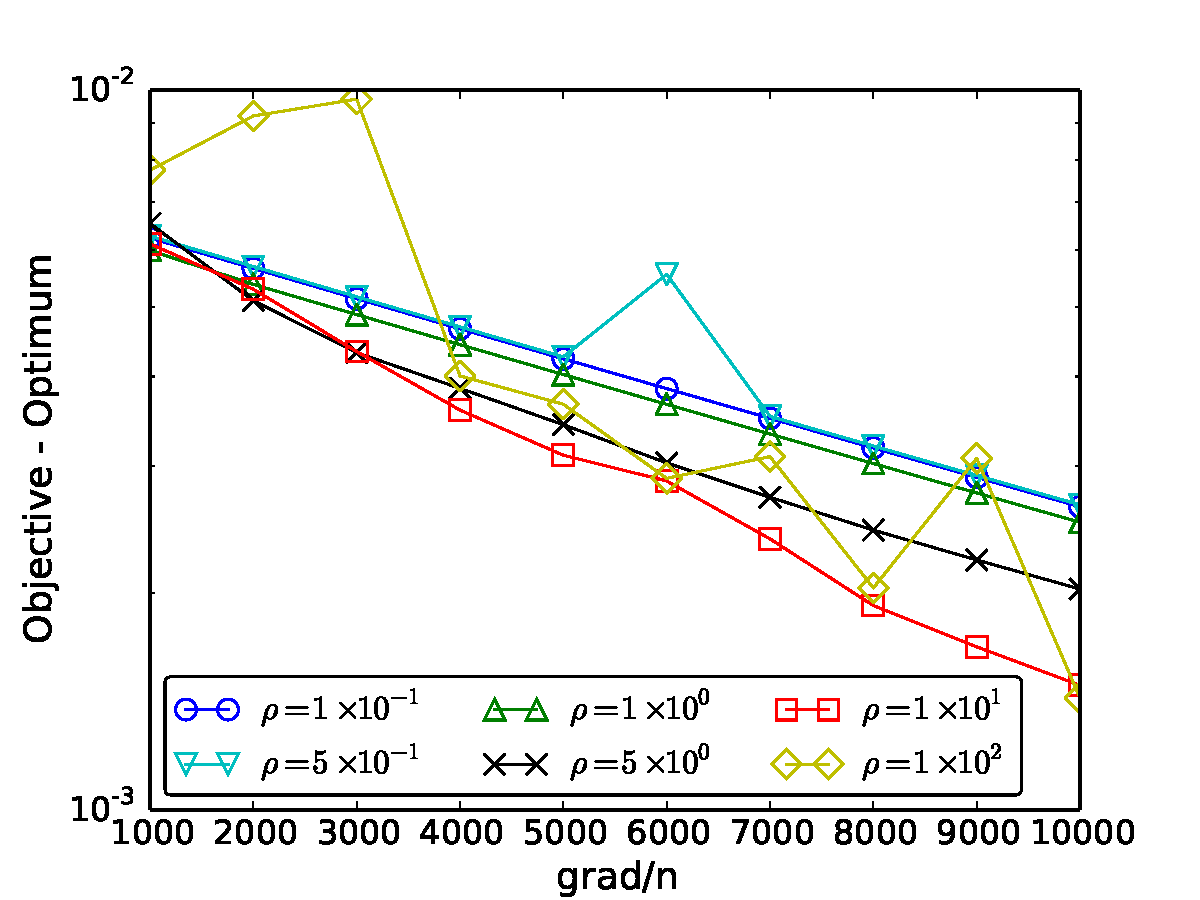
\includegraphics[width=0.5\columnwidth]{figure_space-ga_rho}\label{figure_space-ga_rho}}
\caption{A large $\epsilon$ leads to the fast convergence of the training loss for \emph{sampleVR} when conducting the ridge regression tasks. However, the performance of  \emph{sampleVR} is impaired  due to the increase of variance when $\epsilon$ is set to be too large.}
\label{figure_ridge_regression_rho}
\end{figure*}

%\begin{figure*}[t]
%\centering
%\subfigure[mg]{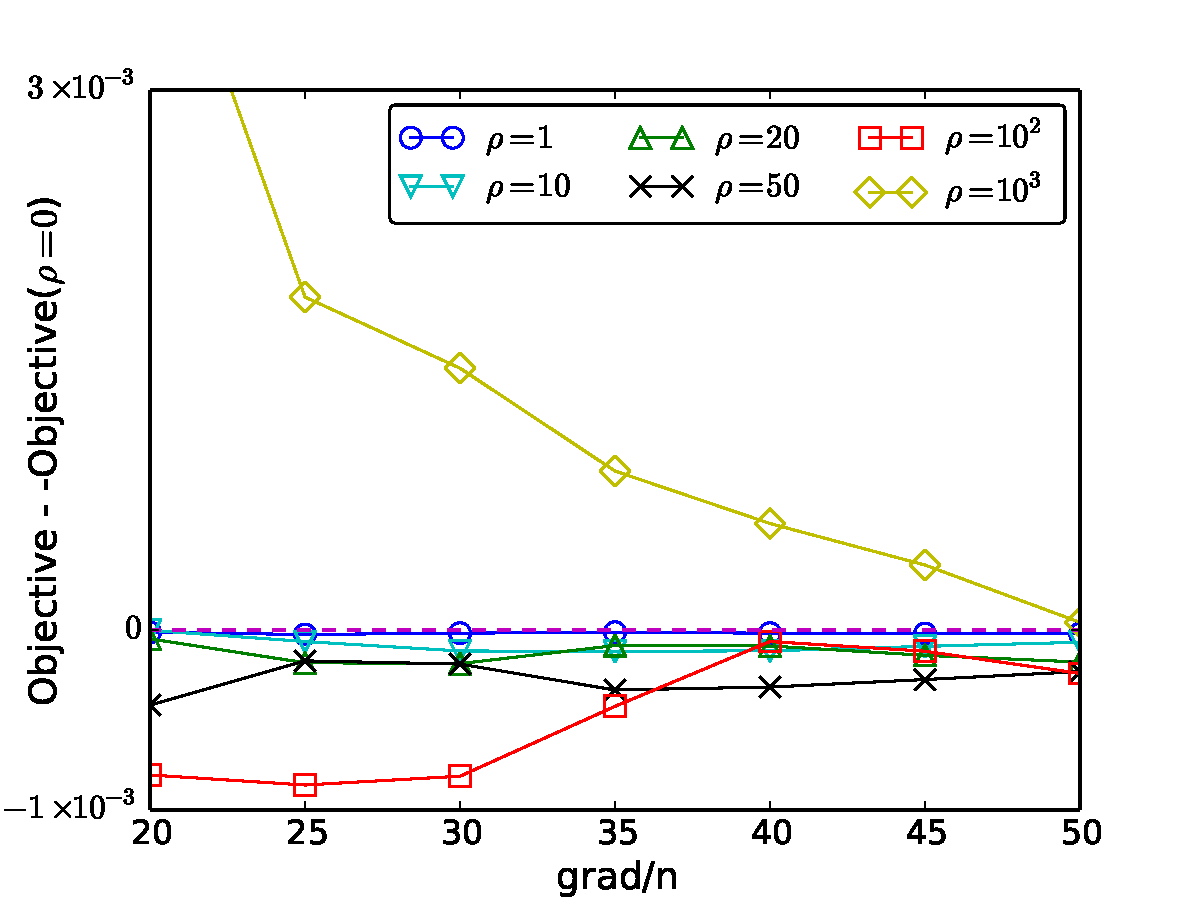
\includegraphics[width=0.5\columnwidth]{figure_mg_rate}\label{figure_mg_rate}}
%\subfigure[cpusmall]{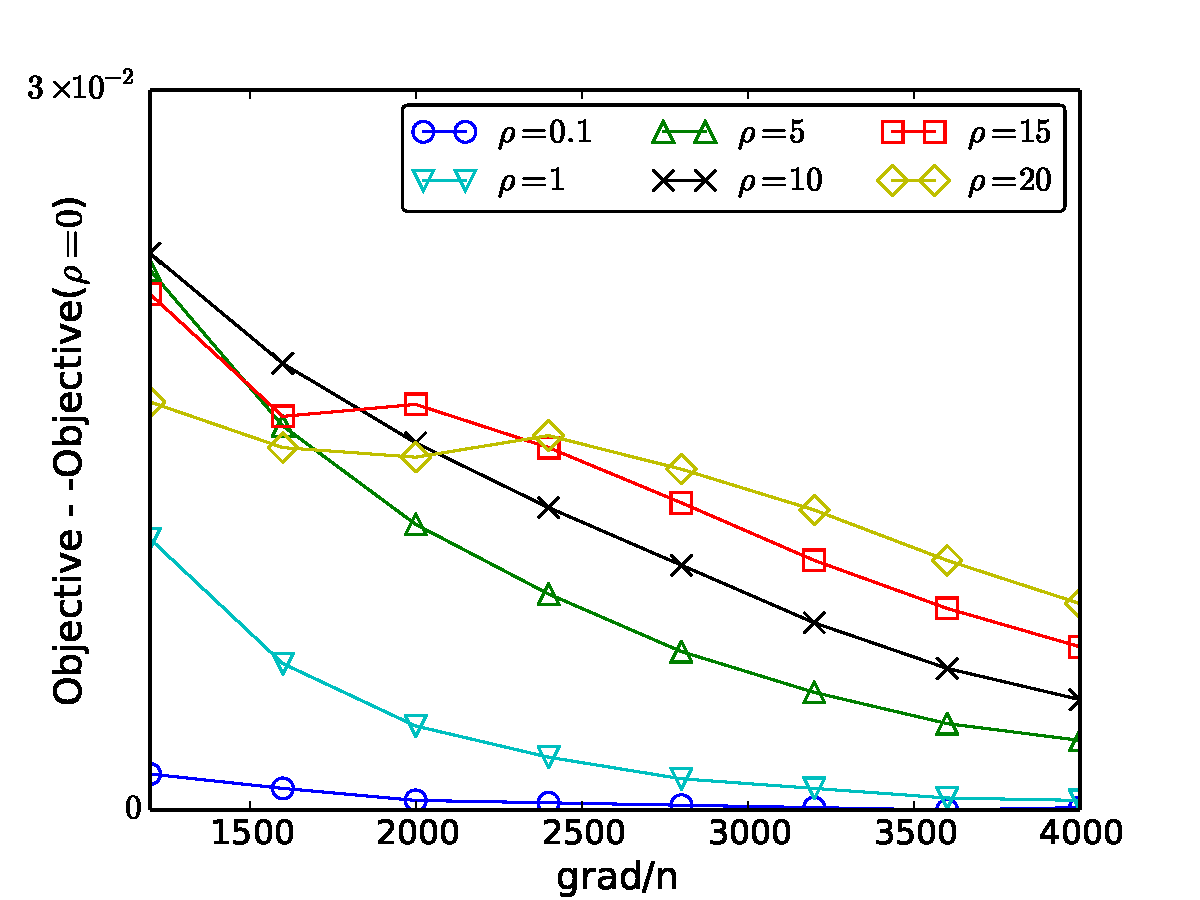
\includegraphics[width=0.5\columnwidth]{figure_cpusmall_rate}\label{figure_cpusmall_rate}}
%\subfigure[yearPredictionMSD]{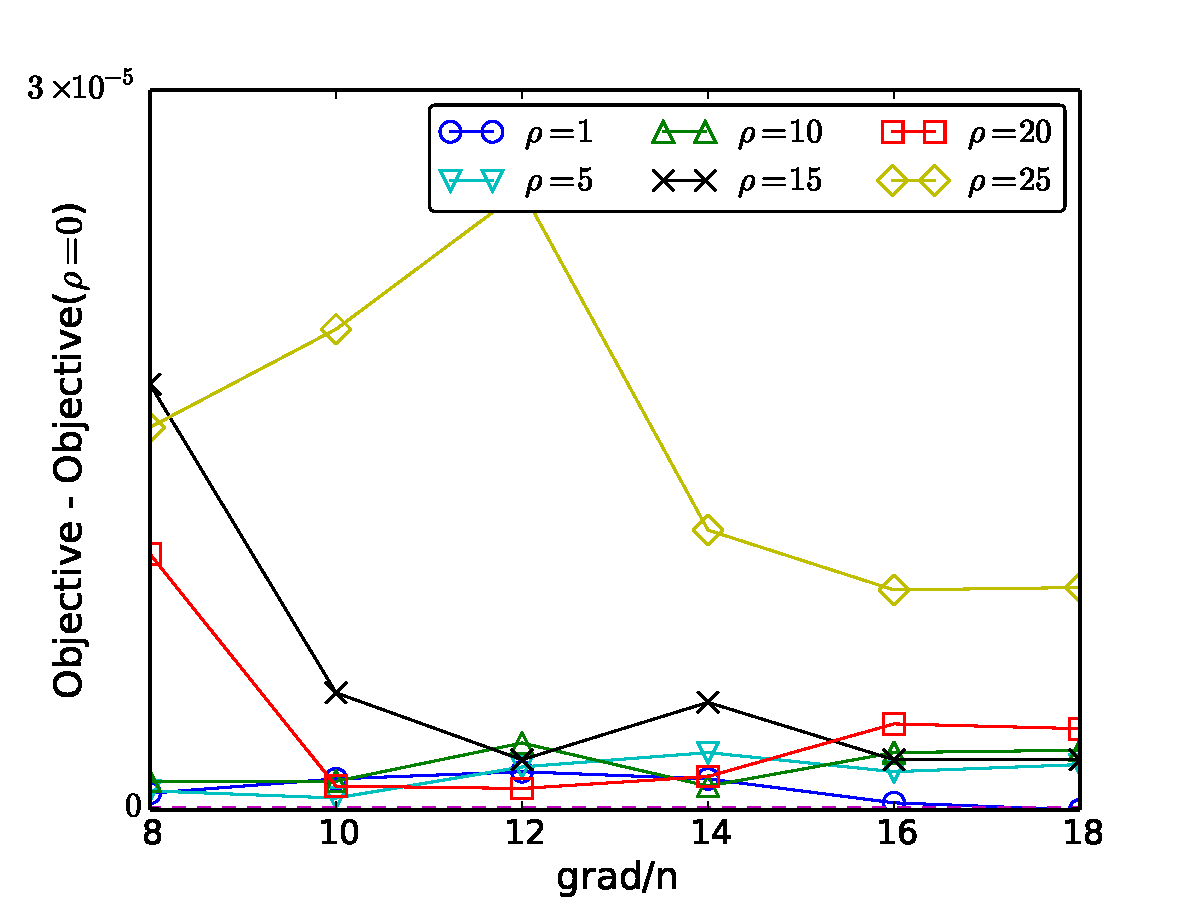
\includegraphics[width=0.5\columnwidth]{figure_year_rate}\label{figure_year_rate}}
%\subfigure[space-ga]{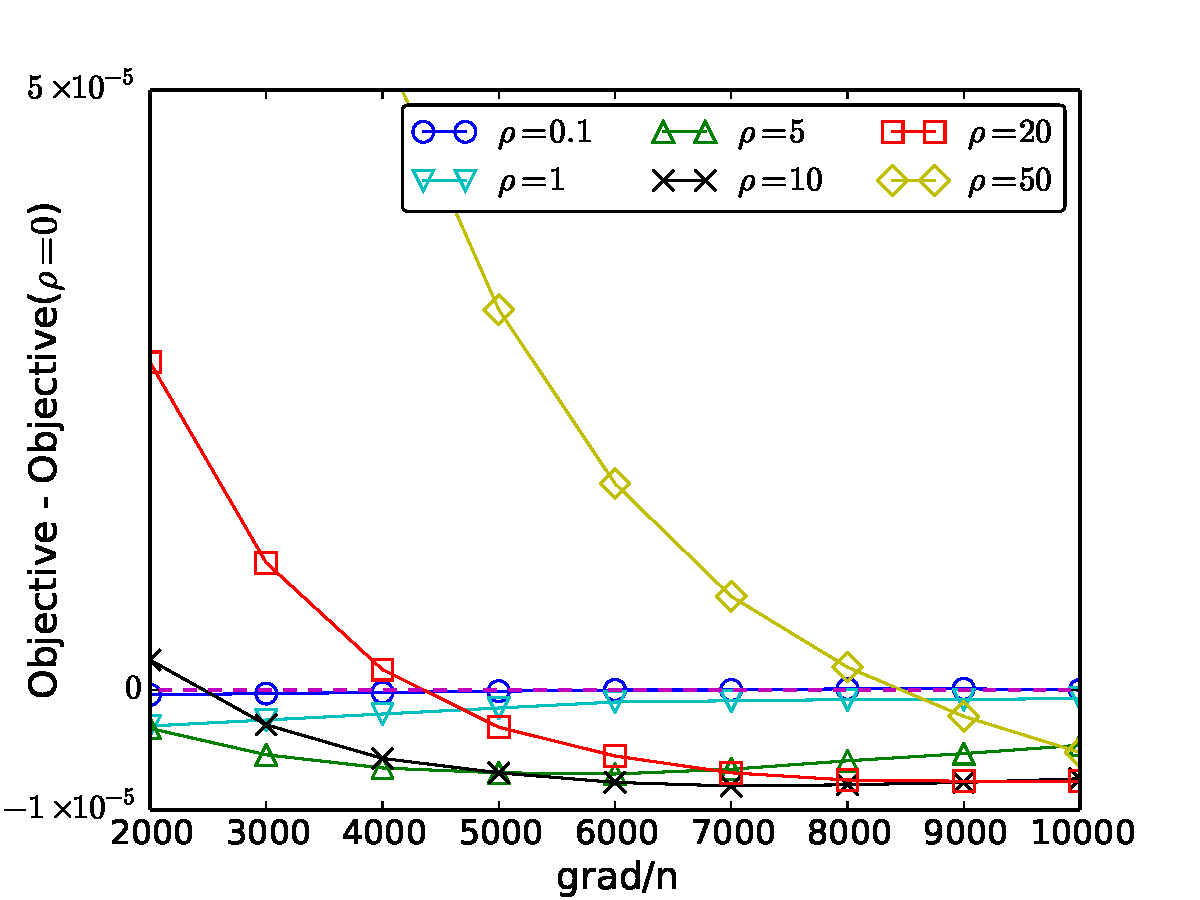
\includegraphics[width=0.5\columnwidth]{figure_space-ga_rate}\label{figure_space-ga_rate}}
%\caption{reuseVR}
%\label{figure_ridge_regression_rate}
%\end{figure*}

\subsection{Experimental settings}
\label{sect_experimental_settings}
The existing variants of SGD with the variance reduction technique, including SVRG, S2GD, SVRG++, cheapSVRG have been used to conduct the performance comparison with our proposed algorithms, i.e. \emph{sampleVR} and \emph{reuseVR}. Those algorithms are evaluated on eight datasets, including ijcnn1, colon-cancer, duke-brease-cancer, a9a, mg, cpusmall, yearPredictionMSD, and space-ga. All of those datasets are public on the LibSVM website \footnote{http://www.csie.ntu.edu.tw/$\sim$cjlin/libsvmtools/datasets/}. First, those algorithms are compared by conducting the $l2$-regularized logistic regression tasks on the datasets: ijcnn1, colon-cancer, duke-breast-cancer, and a9a. The loss function of the $l2$-regularised logistic regression tasks is:
\begin{equation}
\label{standard_sgd}
\min\limits_\omega \frac{1}{n}\sum\limits_{i=1}^n \log(1+e^{-y_i \omega^\mathrm{T} x_i }) + \lambda \parallel \omega \parallel^2
\end{equation}. Second, we compare those algorithms by conducting ridge regression tasks on the other four datasets, i.e. mg, cpusmall, yearPredictionMSD, and space-ga. The loss function of the ridge regression tasks is:
\begin{equation}
\label{standard_sgd}
\min\limits_\omega \frac{1}{n}\sum\limits_{i=1}^n\left(\omega^{\mathrm{T}}x_i-y_i\right)^2 + \lambda \parallel \omega \parallel^2
\end{equation}. We set $\lambda$ to be $10^{-5}$, and the learning rate to be $10^{-4}$ for all the evaluation tests. The epoch size $m^s$ is set to be the size of the training data, i.e. $n$ defaultly.  The x-axis in all the figures  is the computational cost measured by the number of gradient computations divided by  the size of the training data, i.e. $n$. The y-axis in all the figures denotes the training loss residual which is the training loss minus the optimum. Here, the optimum is estimated by running the gradient descent for a long time. The fraction in the bracket of the legend of SVRG++ represents the initial size of the epoch divided by the default size of the epoch. The value in the bracket of the legend of \emph{sampleVR} represents $\epsilon$ according to Algo. \ref{algorithm_estimatevr}.

\subsection{$l2$-regularised logistic regression}
\label{sect_performance_evaluation_convergence}
As illustrated in Fig. \ref{figure_logistic_regression_convergence}, we compare the performance of all the algorithms by conducting the $l2$-regularised logistic regression tasks.  It is obvious that our proposed algorithms, i.e. \emph{sampleVR} and \emph{reuseVR} make the training loss converge faster than other existing algorithms.  The main reason is that  both \emph{sampleVR} and \emph{reuseVR} replaces  the computation of the full gradient with an estimation, and thus get rid of the time-consuming calculations of the gradient significantly.  Additionally, the comparison of the  performance of \emph{sampleVR} with different settings of $\epsilon$ is shown  in Fig. \ref{figure_logistic_regression_rho}. \emph{sampleVR} generally obtains a better performance with a larger $\epsilon$. It is because that the number of the required sampled instances becomes small with a large $\epsilon$ according to Equ. \ref{equ_estimate_samples_lower_bound} and Fig. \ref{figure_estimate_full_gradient}. The computational cost is decreased with a large $\epsilon$, which leads to the acceleration of \emph{sampleVR}. However, as illustrated in Fig. \ref{figure_ijcnn_rho} and \ref{figure_a9a_rho}, if $\epsilon$l is set to be too large, the performance will be impaired due to the variance between the full gradient and the estimation. In specific, a very large $\epsilon$  means that the number of the sampled instances is extremely small. Since the estimation of the full gradient is obtained by the computation of the stochastic gradients according to those instances,  such the estimation has much variance which slows the convergence of the training loss. 

\subsection{Ridge regression}
\label{sect_performance_evaluation_convergence}
As illustrated in Fig. \ref{figure_ridge_regression_convergence}, we report the comparison of the performance by using all the algorithms to  conduct the ridge regression tasks. It is significant that  \emph{reuseVR} makes the loss function converge faster than the existing algorithms. It is because that \emph{reuseVR} uses the average of the stochastic gradients during the iterations of the current epoch to estimate the full gradient for the next epoch, thus leading to  no computational cost of the gradients. Additionally, \emph{sampleVR} has a better performance for the datasets mg, cpusmall, and space-ga than the existing algorithms significantly.  Although \emph{sampleVR} does not outperform other algorithms for the dataset yearPredictionMSD at the beginning of the train process, its performance is comparable to the other algorithms, and finally shows the advantage over most of the existing algorithms. The main reason is that \emph{sampleVR} takes an unbiased estimation of the full gradient, instead of costing much time to compute it. Therefore, \emph{sampleVR} accelerates the convergence of the loss function than other algorithms. As illustrated in Fig. \ref{figure_ridge_regression_rho}, the performance of \emph{sampleVR} has been compared by varying the value of $\epsilon$. It is significant that the variance becomes noticeable with the increase of $\epsilon$. It is because that a large $\epsilon$ leads to a few instances which are sampled in the current epoch according to Equ. \ref{equ_estimate_samples_lower_bound} and Fig. \ref{figure_estimate_full_gradient}. Therefore, the estimation of the full gradient has much variance which slows the convergence of the training loss. Moreover, as illustrated in Fig. \ref{figure_mg_rho}, \ref{figure_cpusmall_rho} and \ref{figure_space-ga_rho}, an extremely small  $\epsilon$  impairs  the performance of \emph{sampleVR}. The reason is that a small $\epsilon$ means that a large number of the instances are sampled for estimating the full gradient, and thus leads to much calculations of gradients. Such a large amount of calculations of gradients cost much time, and make the convergence of the loss function slow down.  



\section{Conclusion}
\label{sect_conclusion}



\bibliography{reference}
\bibliographystyle{aaai}





\end{document}
